\documentclass[11pt,letterpaper]{article}
\usepackage[margin=1in]{geometry}
\usepackage{amsmath,amssymb}
\usepackage{graphicx}
\usepackage{booktabs}
\usepackage[hidelinks]{hyperref}
\usepackage{float}

\setlength{\parindent}{0pt}
\setlength{\parskip}{0.6em}
\setcounter{tocdepth}{1}

\newcommand{\tasksection}[2]{
    \clearpage
    \phantomsection
    \section*{#1: #2}
    \addcontentsline{toc}{section}{#1: #2}
}

\title{Project 2 Report\\[0.4em]
    \large CMPEN/EE 454}
\author{Mingcheng Liang, TianKuo Liao, Yuxin Liu\\}
\date{2026/10/27}

\begin{document}

\maketitle
\tableofcontents

\tasksection{Task 3.1}{Camera Parameters}

\subsection*{Internal and External Parameters}
Task 3.1 involves determining what the fields of the input camera parameter structure mean in regards to the pinhole camera model parameters that were discussed in class lectures.

Each of the camera structures stores the following fields:

\medskip

Internal (intrinsic) parameters, describes the camera itself:
\begin{itemize}
    \item Focal Length $(f)$
    \item Principal Point $(c_x, c_y)$
    \item Aspect Ratio $(a)$
    \item Skew $(s)$
\end{itemize}

External (extrinsic) parameters describe where the camera is in the world:
\begin{itemize}
    \item Position, the camera center $(C)$
    \item Orientation, a unit quaternion that corresponds to the $3\times3$ rotation matrix \texttt{Rmat} ($R$).
\end{itemize}
We use \texttt{Rmat}, not the quaternion, in all projection equations.

\subsection*{Building $K_{\text{mat}}$}
The internal parameters \texttt{focal length $(f)$}, \texttt{principal point $(c_x, c_y)$}, \texttt{aspect ratio $(a)$}, and \texttt{skew $(s)$} combine into:

\[
K_{\text{mat}} = \begin{bmatrix}
    f a & s & c_x \\ 0 & f & c_y \\ 0 & 0 & 1
\end{bmatrix}
\]

\medskip

Our code builds this matrix from the fields and prints the difference from the stored camera 1 and 2 \texttt{Kmat} and calculated \texttt{Kmat}. The difference is exactly zero for both cameras.

For camera 1: 
\begin{center}
    $f=1560.6793$
    \\$(c_x, c_y)=(967.5391, 548.7386)$
    \\$a=1.0000$
    \\$s=0.0000$
\end{center}

For camera 2: 
\begin{center}
    $f=1527.9015$
    \\$(c_x, c_y)=(969.8920, 549.8908)$
    \\$a=1.0000$
    \\$s=0.0000$
\end{center}

\subsection*{Building $P_{\text{mat}}$}
The external parameters \texttt{Rmat} and \texttt{position} combine into:
 \[
 P_{\text{mat}} = \begin{bmatrix}
     R & -RC
 \end{bmatrix}
 \]
 which maps a world point into camera coordinates, $X_{cam}=R(X-C)$. The stored \texttt{Pmat} does not contain \texttt{Kmat}, so the full projection is $\texttt{Kmat}\cdot\texttt{Pmat}$.

 In MATLAB, in order to verify that the camera location and \texttt{Rmat} combined in the expected way, our code forms $[\,R\;\;-RC\,]$ from \texttt{Rmat} and \texttt{positon} and prints its difference from the stored \texttt{Pmat}. For both cameras every entry differs by at most about $10^{-13}$, which is zero to floating-point precision. 

 \subsection*{Camera Location}
 The camera location is the \texttt{position} field, in millimeters in the world frame.
 \\For camera 1: 
\begin{center}
    Position  $(C) = (-4479.6412,\ 5524.6708, \ 1899.0398)$
\end{center}

For camera 2: 
\begin{center}
    Position  $(C) = (4416.8864,\ 5513.7913, \ 1788.9126)$
\end{center}


\tasksection{Task 3.2}{Projection of 3D Points}
\label{sec:task3-2}

\subsection*{Projection model}

We projected the 39 mocap points into each image with the pinhole chain from class lecture. A world point $[X,Y,Z]^T$ is converted to homogeneous form $\Tilde{X}=[X,Y,Z,1]^T$, and its pixel location is:

\[
\Tilde{x} = \texttt{Kmat}\cdot\texttt{Pmat}\cdot\tilde{X}
\qquad
(u,v) = \left(\frac{\Tilde{x}_1}{\Tilde{x}_3},\ \frac{\Tilde{x}_2}{\Tilde{x}_3}\right)
\]

\medskip

Here \texttt{Pmat} $=[\,R \;\; -RC]$ maps the world point into camera coordinates, $X_{cam}=R(X-C)$ (refer to task 3.1), and \texttt{Kmat} maps camera coordinates into pixels. This is a matrix product of sizes $(3\times3)(3\times4)(4\times1)$. The division by the third coordinate is the homogeneous-to-pixel step. 

\subsection*{Implementation}
The function \texttt{task 3\_2} is written from scratch using only matrix multiplication and element-wise division, with no toolbox projection functions. 

The $3\times39$ array of mocap points is padded with a row of ones to make a $4\times39$ homogeneous array. A single matrix product $\texttt{Kmat}\, \texttt{Pmat}$ times this array projects all 39 points at once, and the first two rows are then divided by the third row. This is done separately for camera 1 and camera 2. 

The function returns two $2\times39$ arrays of pixel coordinates. These are the 39 point correspondences used late for triangulation and for evaluating the fundamental matrices. The function also draws the projected points on the two images. 

\subsection*{Results}
Figure~\ref{fig:task3-2} shows the projected points (red) overlaid on the two corrected images. 

\begin{figure}[H]
    \centering
    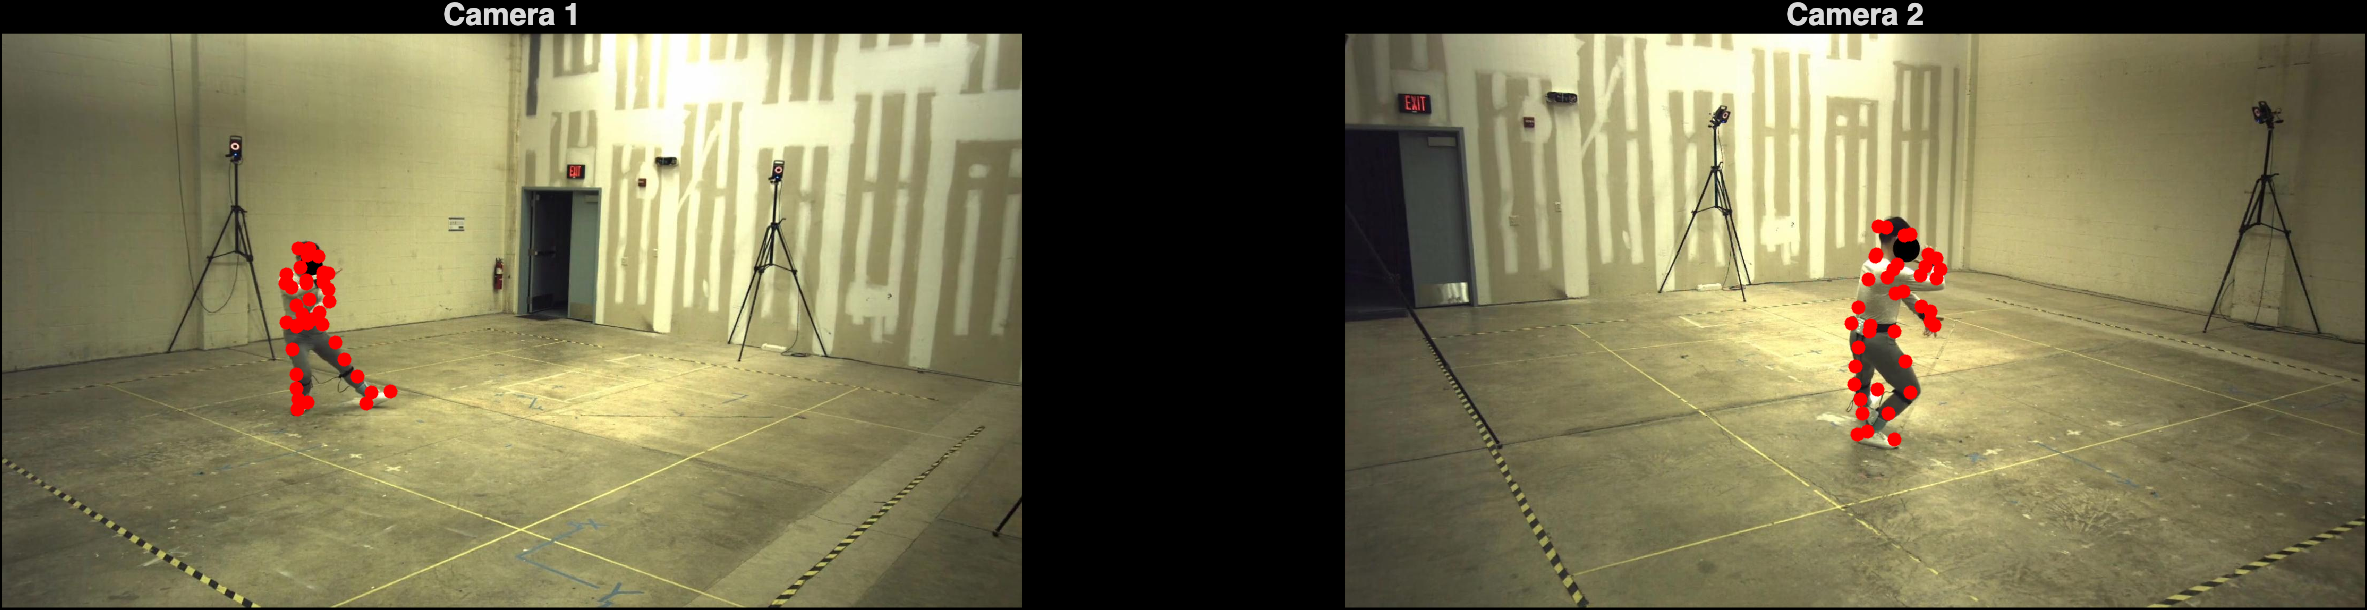
\includegraphics[width=\linewidth]{task3_2_projection.png}
    \caption{Projected mocap points (red) on camera 1 (left) and camera 2 (right).}
    \label{fig:task3-2}
\end{figure}

\medskip

In both views the projected points trace the performer's legs, torso, arms, and head, and the overall shape matches the pose of the person in the image, so the projection is correct for both cameras. Some markers indicate lying on the side of the body facing away from the camera, so no marker is visible there in the image, but the points still land on person's body outline. 

\tasksection{Task 3.3}{3D Reconstruction by Triangulation}
\label{sec:task3-3}

\subsection*{Objective and projection model}
Task 3.2 produces two sets of corresponding pixel locations by projecting the 39 mocap points into the two camera views. In this task, each pair is used to reconstruct a 3D point, which is then compared with its original mocap position.

For camera $j\in\{1, 2\}$, use the full pixel projection matrix:
\[
    P_j = K_j \, \texttt{Pmat}_j \in \mathbb{R}^{3 \times 4}.
\]
Here, $K_j$ is the intrinsic matrix and $\texttt{Pmat}_j$ is the world-to-camera extrinsic matrix. A world point $\widetilde{\mathbf{X}}=[X,Y,Z,1]^T$ and its corresponding pixel $\widetilde{\mathbf{x}}_j=[u_j,v_j,1]^T$ satisfy:
\[
    \lambda_j \widetilde{\mathbf{x}}_j = P_j \widetilde{\mathbf{X}},
    \qquad j = 1, 2,
\]
where $\lambda_j$ is the projective scale. 

Ideally, the two back-projected rays intersect at the original 3D point. However, measurement noise or numerical errors may prevent an exact intersection. We therefore reconstruct the 3D point using linear triangulation based on the Direct Linear Transformation (DLT) method, with the homogeneous system solved using Singular Value Decomposition (SVD).

\subsection*{Linear triangulation and SVD implementation}

Write the rows of $P_j$ as $p_{j1}^T , p_{j2}^T , p_{j3}^T$. Eliminating $\lambda_j = p_{j3}^T \widetilde{\mathbf{X}}$ gives two linear constraints per camera:
\[
    (u_j p_{j3}^T - p_{j1}^T)\widetilde{\mathbf{X}}=0,
    \qquad
    (v_j p_{j3}^T - p_{j2}^T)\widetilde{\mathbf{X}}=0.
\]
Combining both views yields a $4\times4$ homogeneous system,
\[
    A\widetilde{\mathbf{X}}=0,
    \qquad
    A=\begin{bmatrix}
        u_1 p_{13}^T - p_{11}^T\\
        v_1 p_{13}^T - p_{12}^T\\
        u_2 p_{23}^T - p_{21}^T\\
        v_2 p_{23}^T - p_{22}^T
    \end{bmatrix}.
\]
In an ideal noise-free and non-degenerate case, $A$ has rank three and its null space determines the point up to scale. But with numerical error or noisy coordinates, we need to solve the constrained algebraic least-squares problem:
\[
    \widehat{\mathbf{h}} = \underset{\| \mathbf{h} \|_2 = 1}{\operatorname{argmin}}\| A \mathbf{h} \|_2^2.
\]
The constraint excludes the trivial solution. 

Let
$A = U \Sigma V^T$ with singular values $\sigma_1 \geq \sigma_2 \geq \sigma_3 \geq \sigma_4 \geq 0$. Since $A \mathbf{v}_k = \sigma_k \mathbf{u}_k$, the minimum is attained by
$\widehat{\mathbf{h}}=\mathbf{v}_4$, the last column of $V$.

The resulting homogeneous solution is converted to Euclidean 3D coordinates by:
\[
\widehat {\mathbf{X}} = 
\left[
\frac{h_1}{h_4},
\frac{h_2}{h_4},
\frac{h_3}{h_4}
\right]^T.
\]

This produces the reconstructed 3D point in the world coordinate.

\clearpage

\subsection*{Verification against the mocap points}
To verify reconstruction, we pass the two projected point arrays from Task 3.2 in their original correspondence order to the triangulation function. The output $\widehat{\mathbf{X}}_i$ is compared with the corresponding original point $\mathbf{X}_i$ in \texttt{mocap\_data.pts3D}. The quantitative measure is the mean squared distance:
\[
    \mathrm{MSE} = \frac{1}{n} \sum_{i=1}^{n} \left\| \widehat{\mathbf{X}}_i - \mathbf{X}_i \right\|_2^2
\]

The MSE has units of squared world-coordinate units.

\begin{center}
\begin{tabular}{lc}
\toprule
Quantity & Result \\
\midrule
Number of mocap points & 39 \\
Mean squared reconstruction error & $2.58\times10^{-19}$ mm$^2$ \\
\bottomrule
\end{tabular}
\end{center}

Because the image locations were generated from the same cameras and original 3D points, without added measurement noise, the MSE is expected to be very close to zero, with any small residual arising from floating-point arithmetic.

\tasksection{Task 3.4}{Scene Measurements}
\label{sec:task3-4}
\subsection*{Plane fitting}

Given $m\ge 3$ non-collinear points $p_i$, we find the least-squares plane
$Ax+By+Cz+D=0$ with unit normal $n=[A,B,C]^T$. The distance from $p_i$ to
the plane is $d_i = n^Tp_i + D$. Setting the derivative of
$\sum_i d_i^2$ with respect to $D$ to zero gives $D=-n^T\bar{p}$, where
$\bar{p}$ is the mean of the points, so the plane passes through the
centroid.

\medskip

Let $M$ be the matrix whose rows are $(p_i-\bar{p})^T$. Then
$\sum_i d_i^2 = \|Mn\|_2^2$, which is minimized over unit vectors $n$ by
the right singular vector of $M$ with the smallest singular value (the last
column of $V$ in $M=U\Sigma V^T$). The function \texttt{fit\_plane}
implements this.

\subsection*{Floor Plane}
We clicked 3 points on the floor in each image:

\begin{figure}[H]
    \centering
    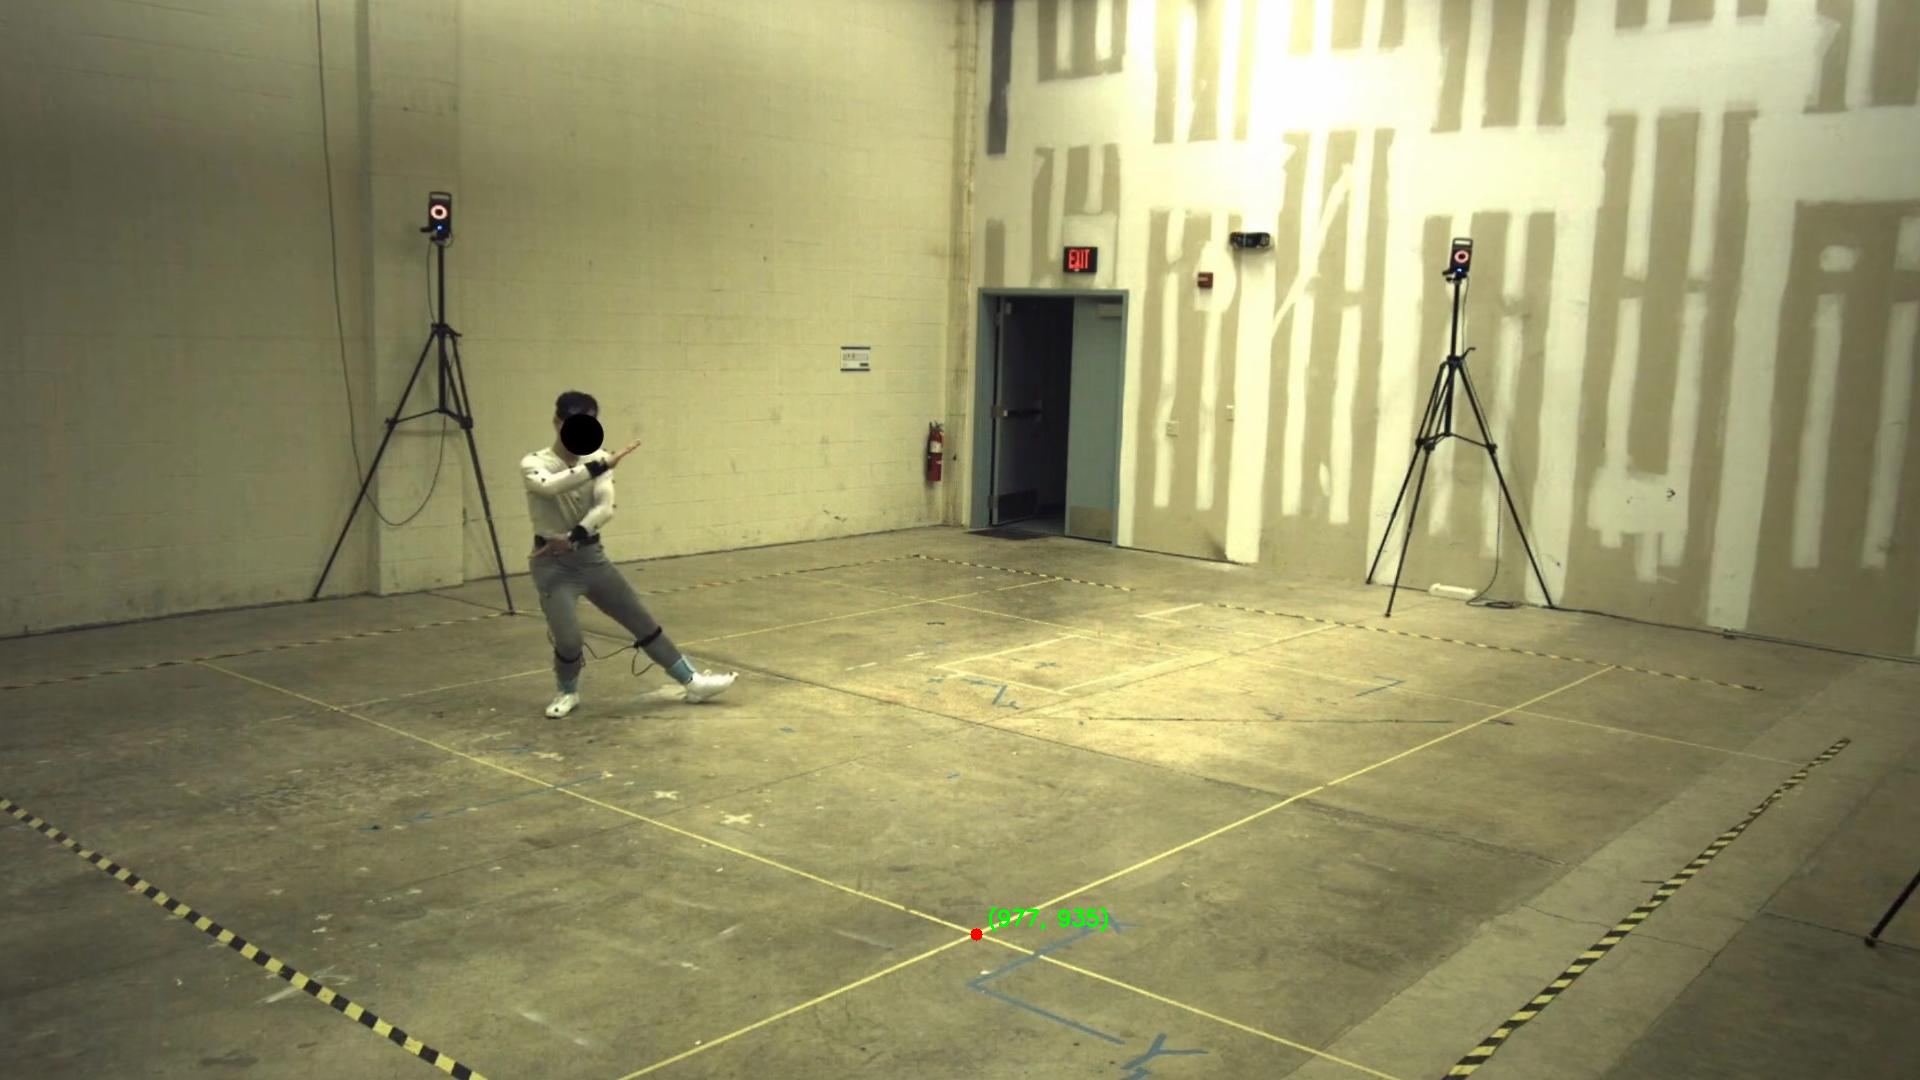
\includegraphics[width=0.32\linewidth]{img1_pt1.png}
    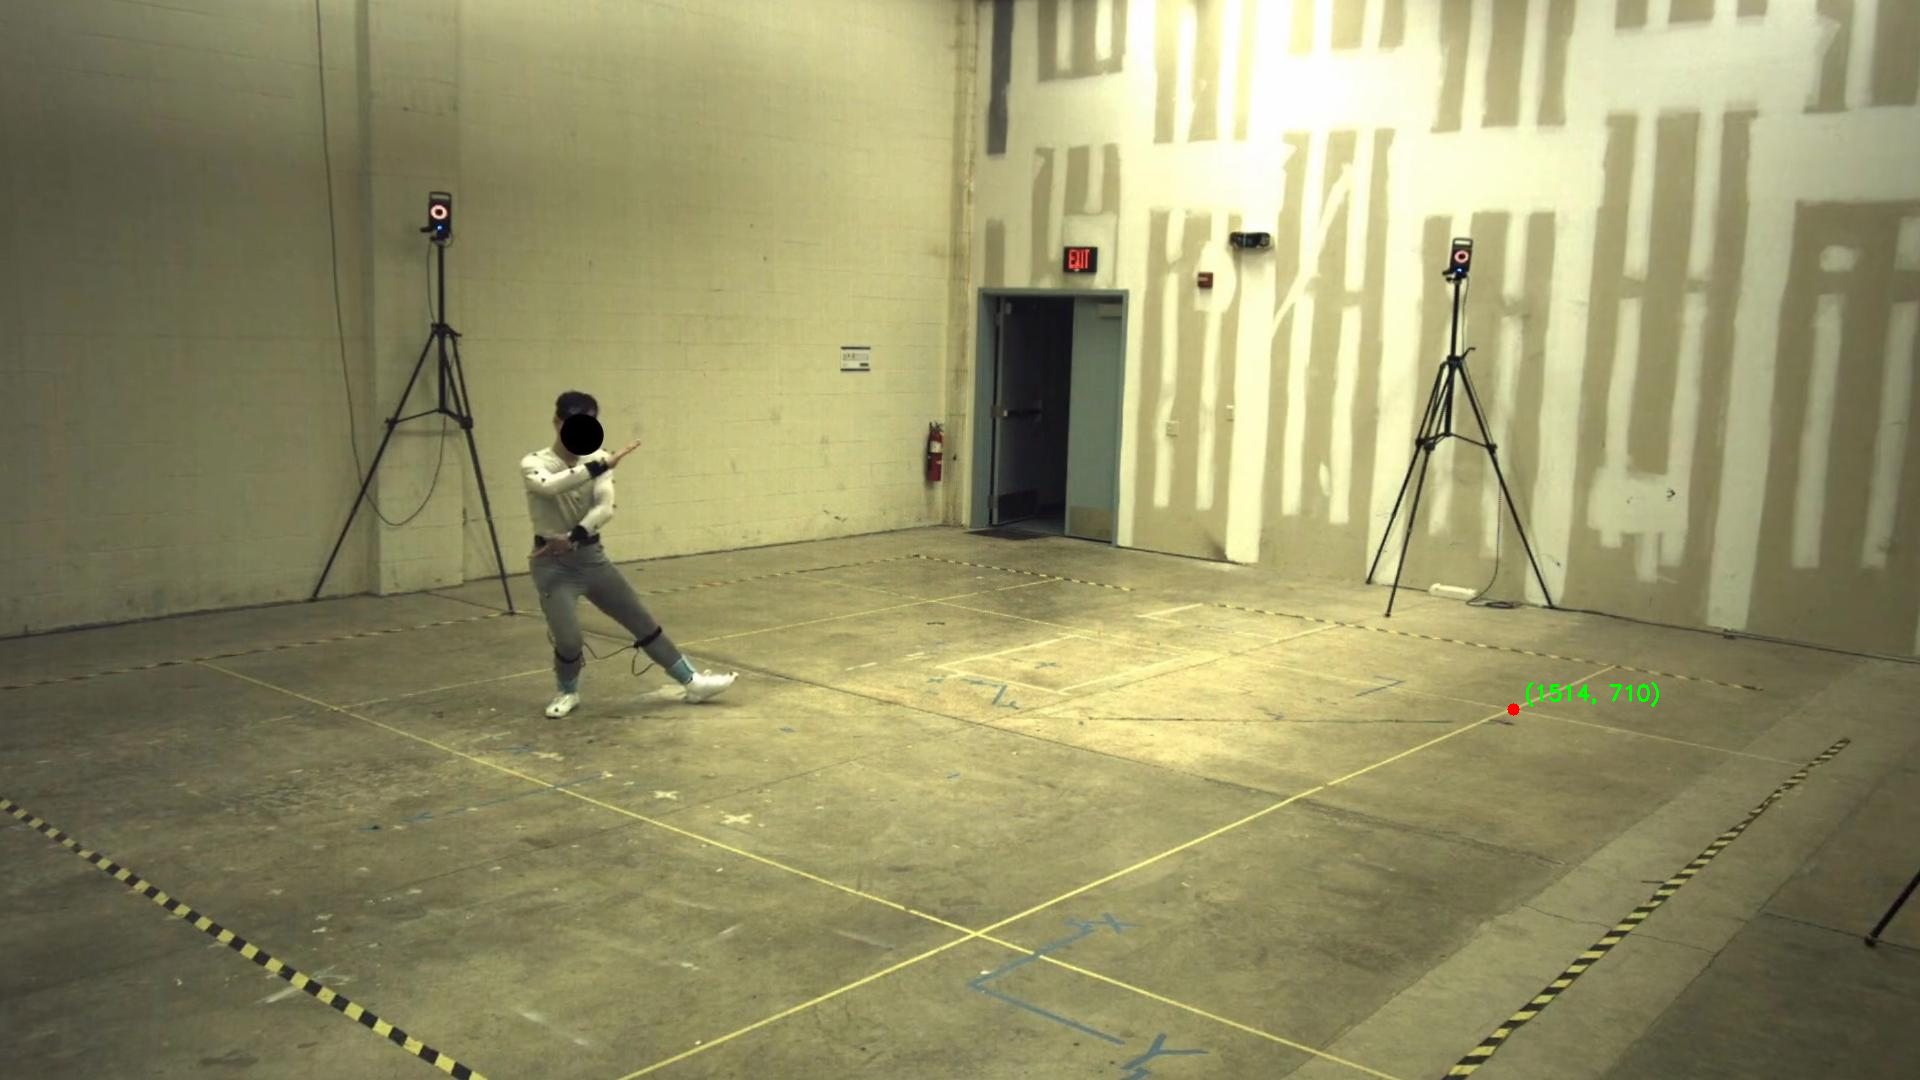
\includegraphics[width=0.32\linewidth]{img1_pt2.png}
    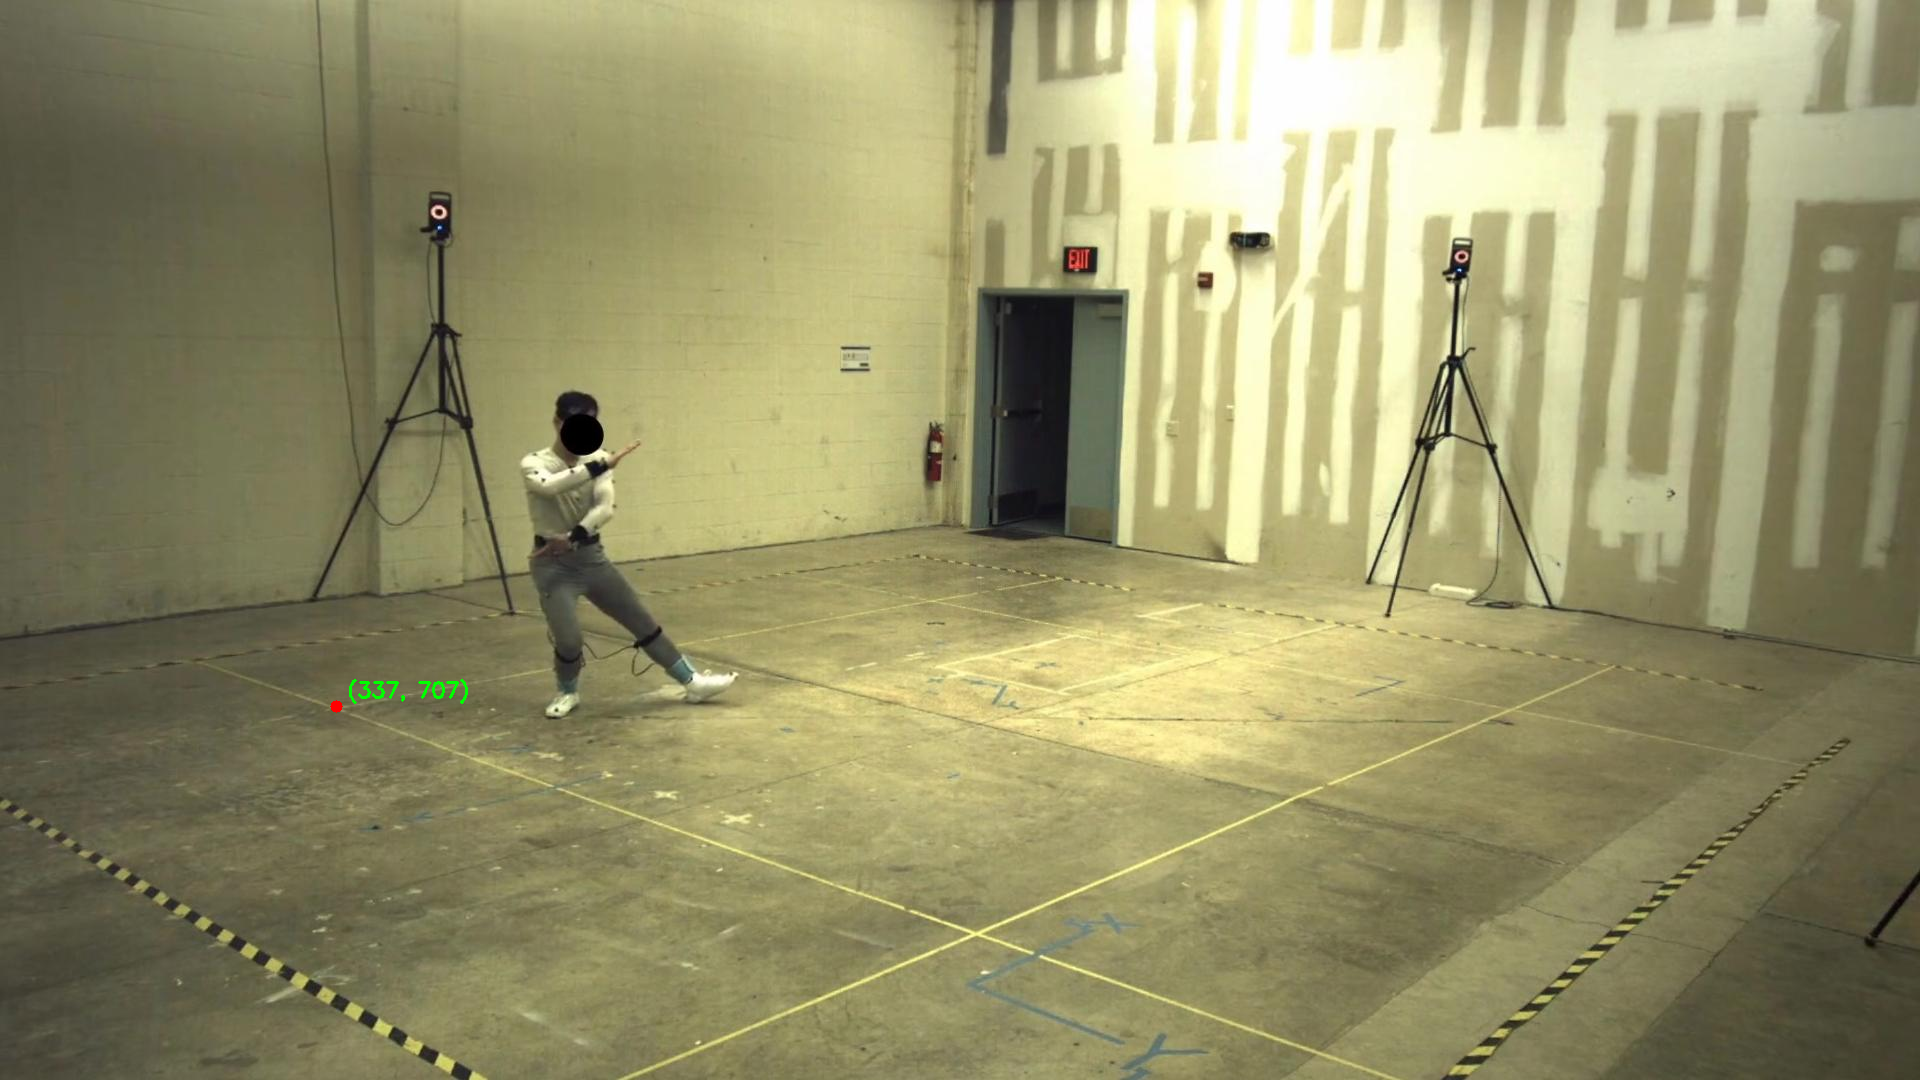
\includegraphics[width=0.32\linewidth]{img1_pt3.png}

    \medskip

    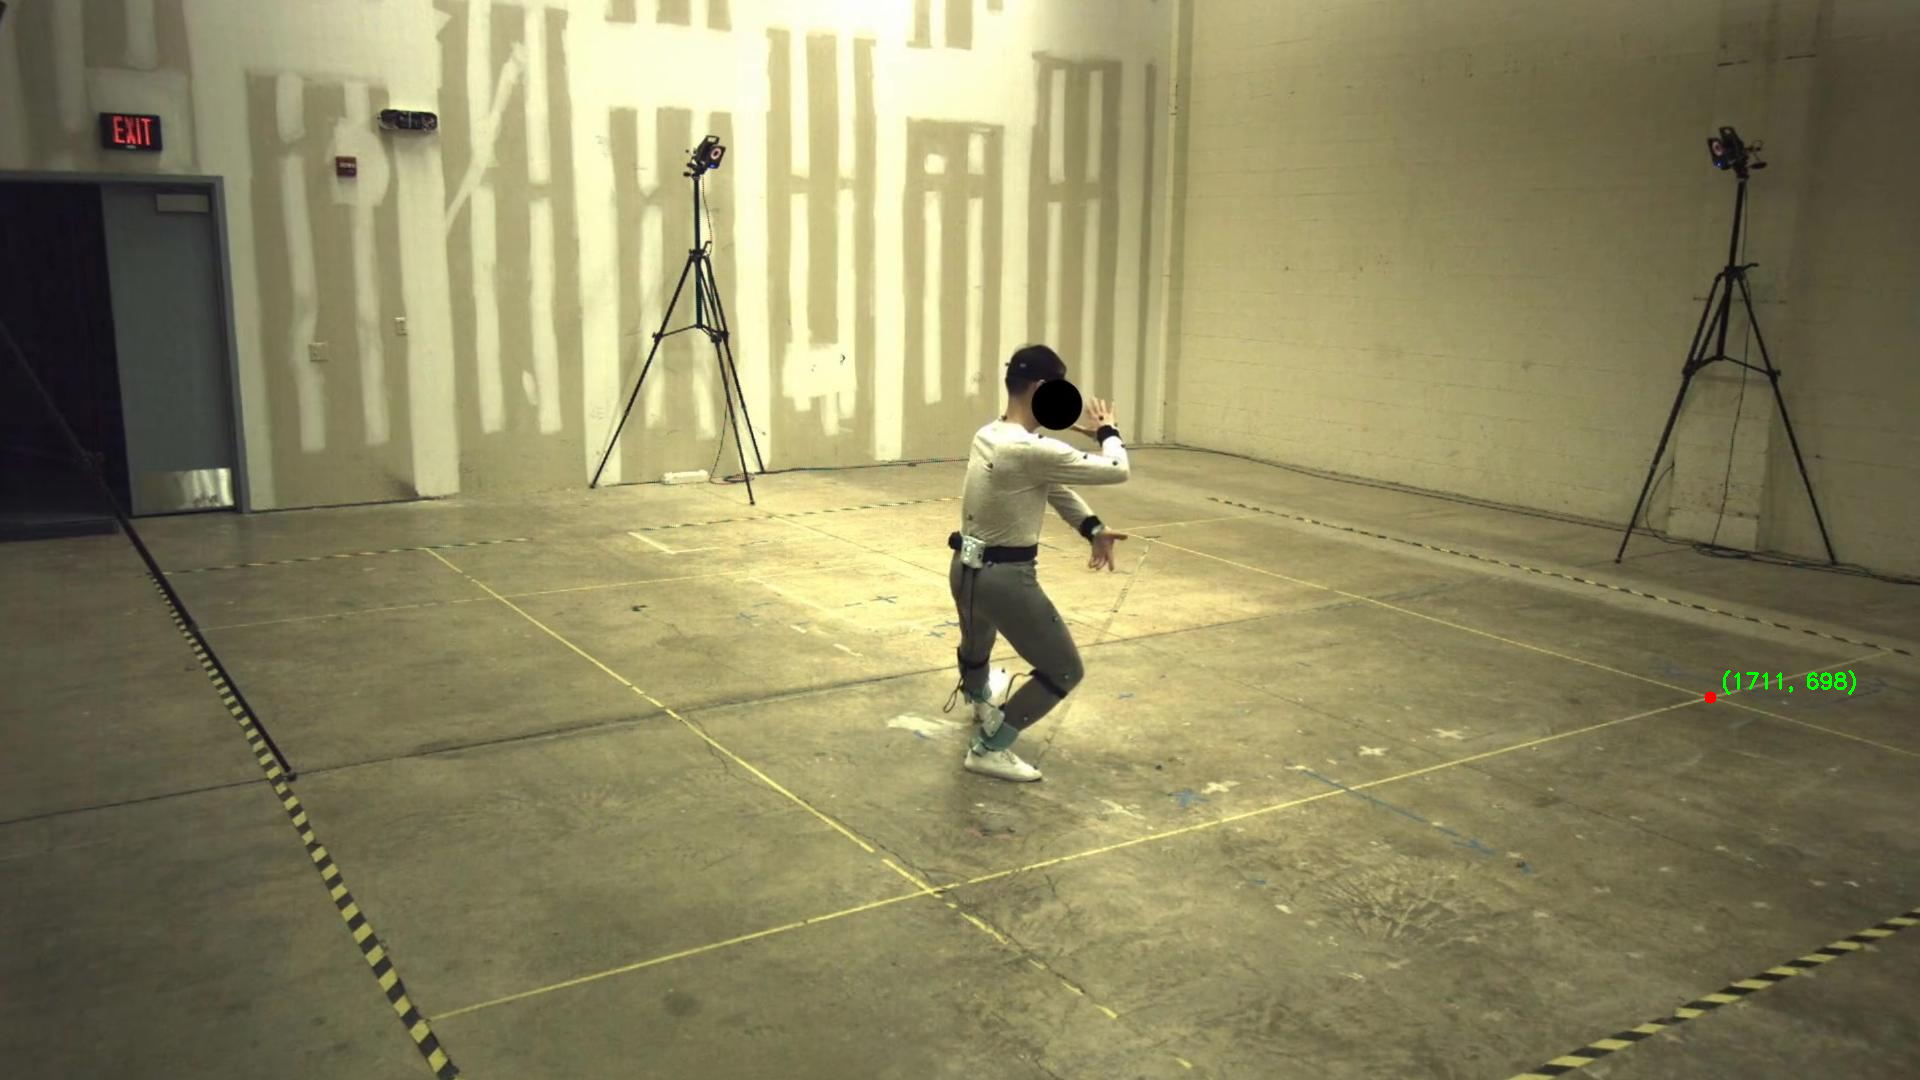
\includegraphics[width=0.32\linewidth]{img2_pt1.png}
    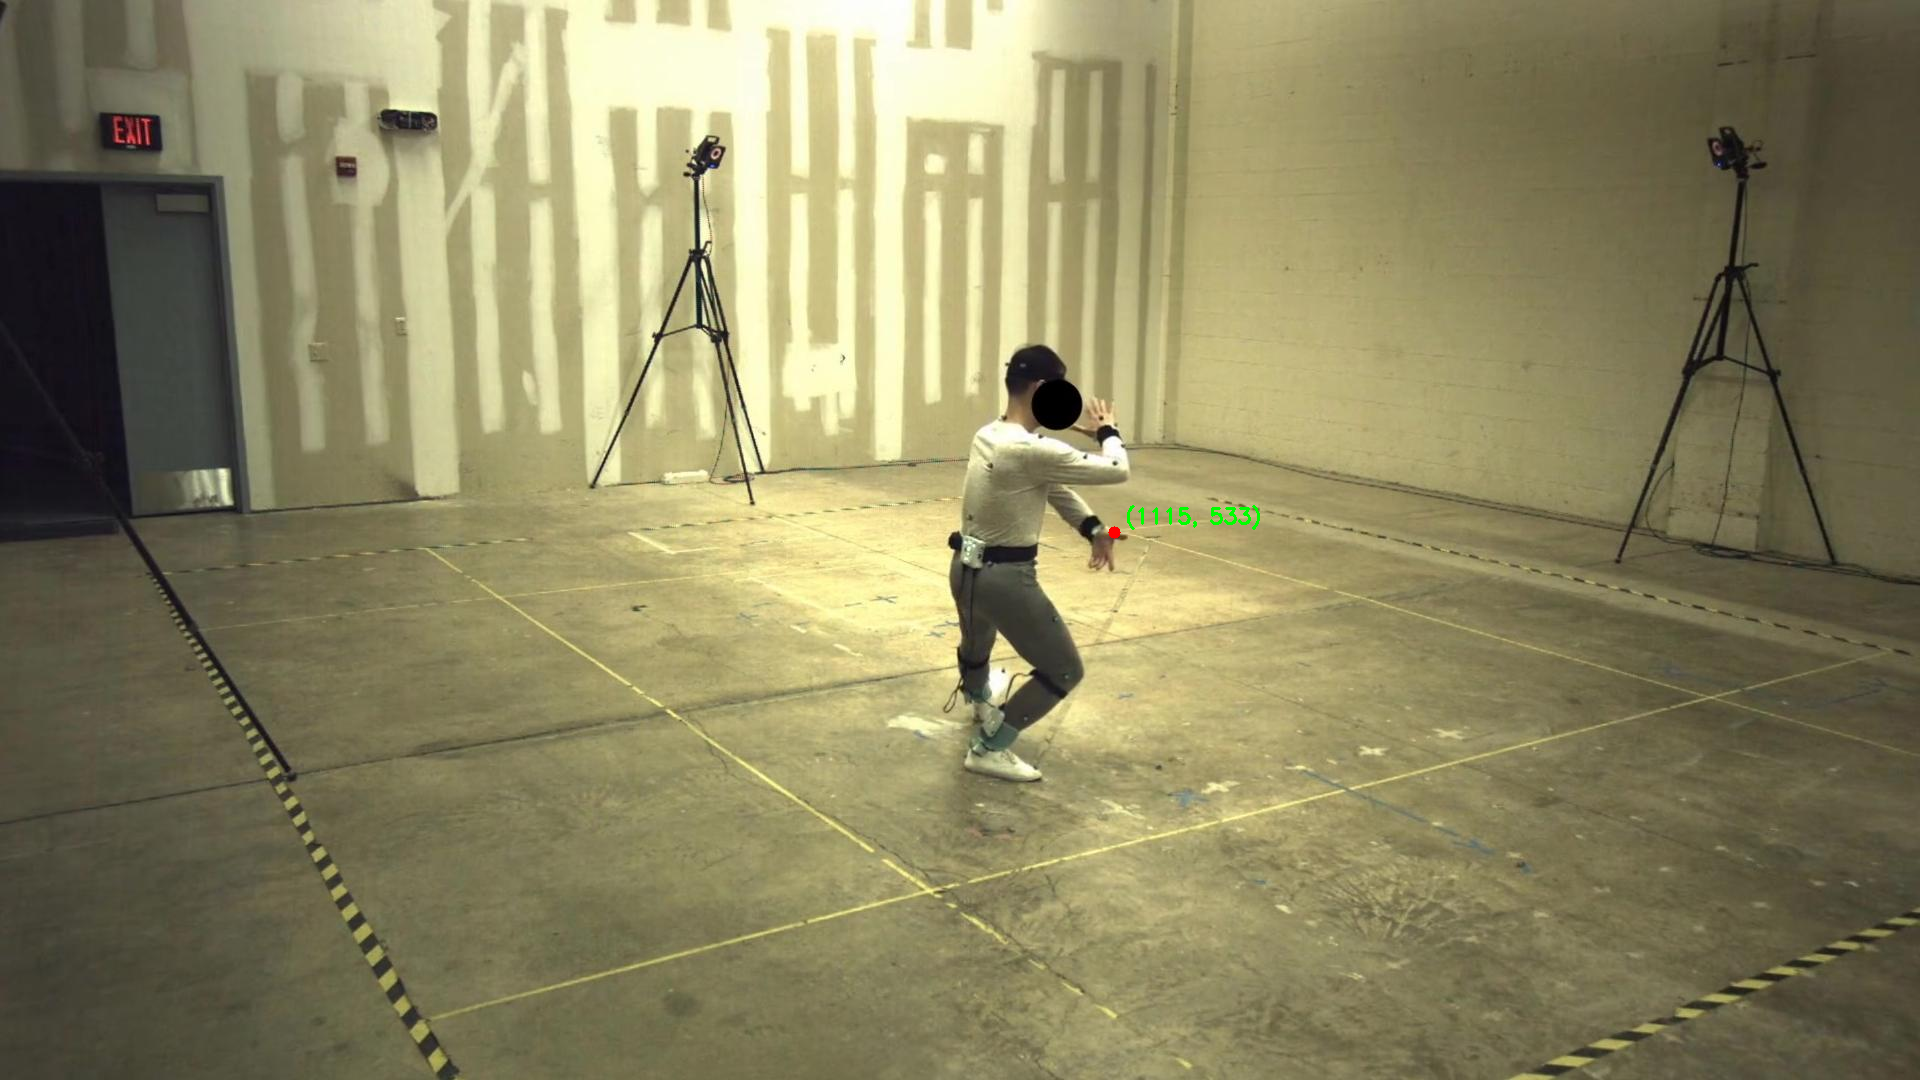
\includegraphics[width=0.32\linewidth]{img2_pt2.png}
    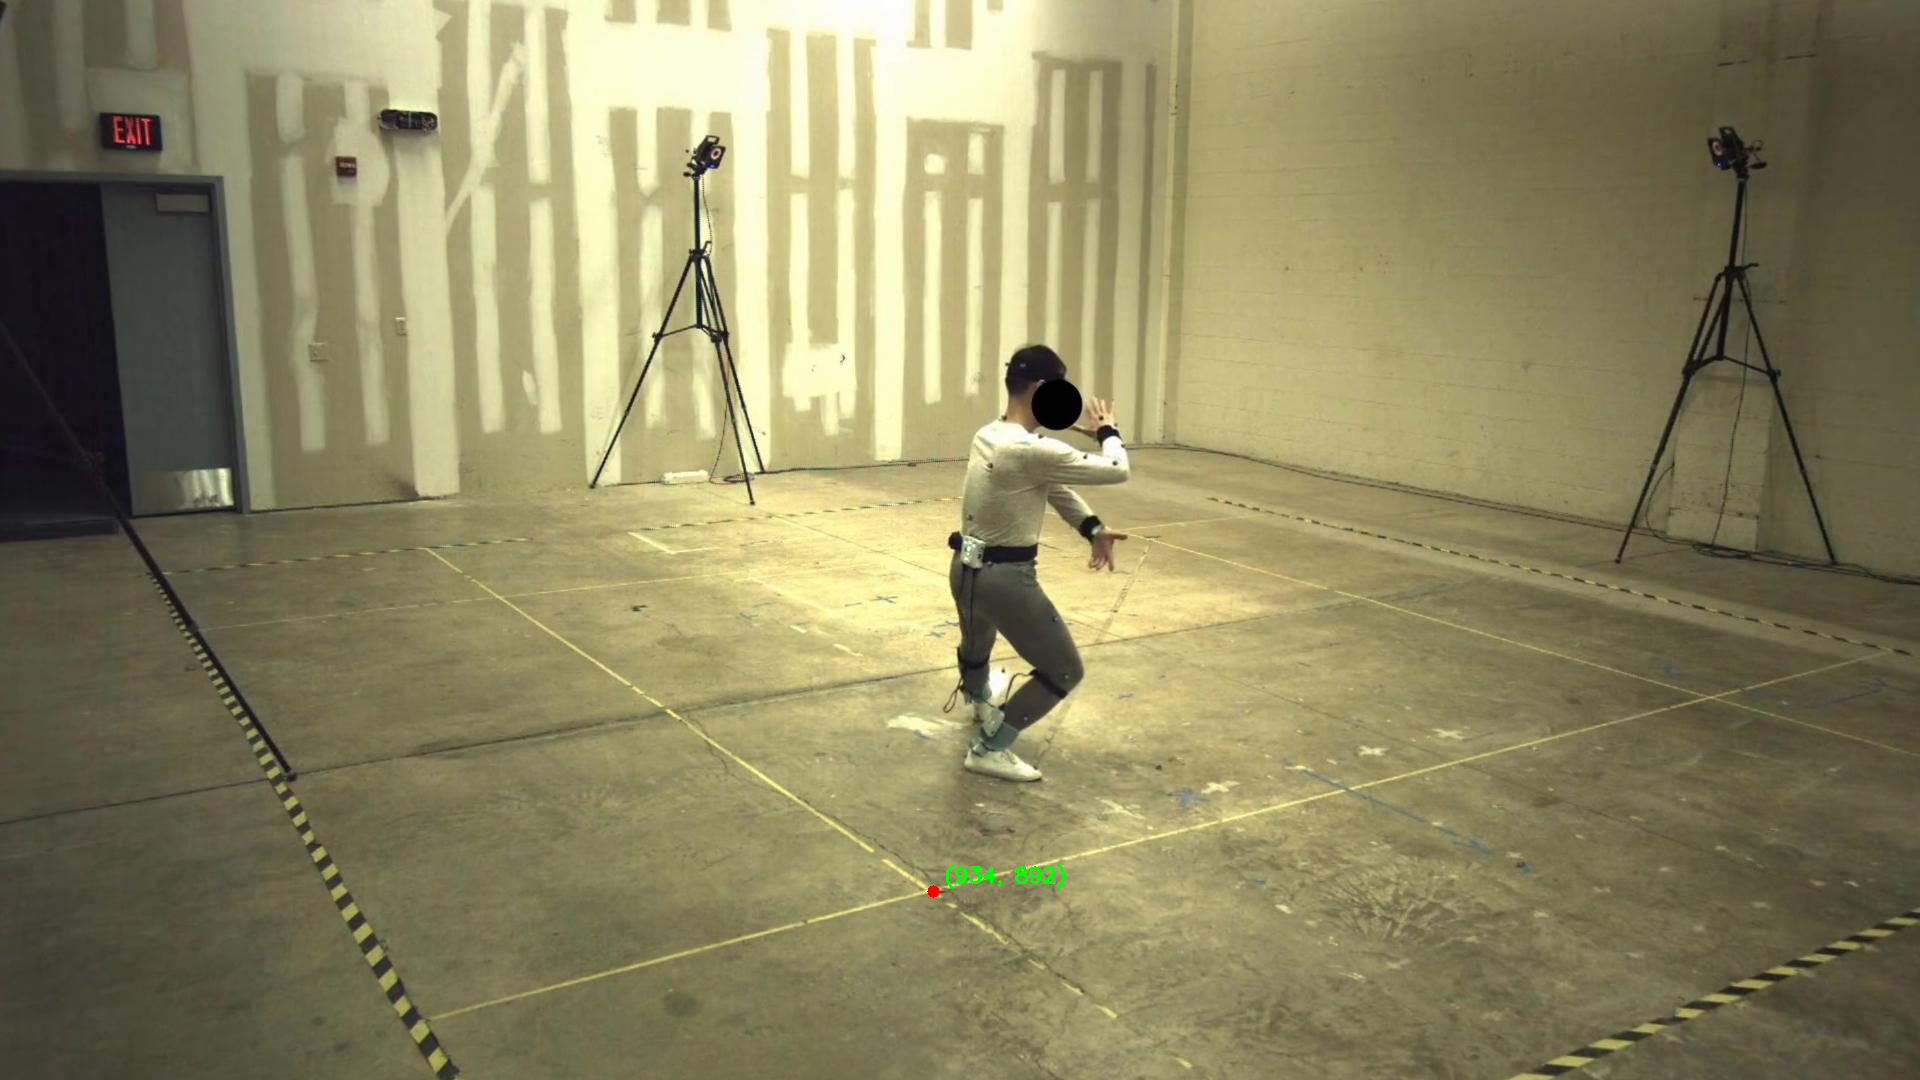
\includegraphics[width=0.32\linewidth]{img2_pt3.png}
    \caption{Floor points clicked in image 1 (top row) and image 2 (bottom row).}
    \label{fig:task3-4-floor}
\end{figure}

The fitted floor plan is:
\[
Floor plane: -0.009683 x +0.0001318 y -1.0000 z -15.35 = 0
\]
its normal makes an angle of $0.55^\circ$ with the $Z$ axis, and the plane sits at $Z\approx -15$ mm. The mean squared $Z$ value of the three floor points is 452.23 mm $^2$ (about 21 mm RMS), consistent with the hand-clicking error. The computed floor plane is therefore, to good approximation, the plane $Z=0$.

\subsection*{Wall Plane}

\begin{figure}[H]
    \centering
    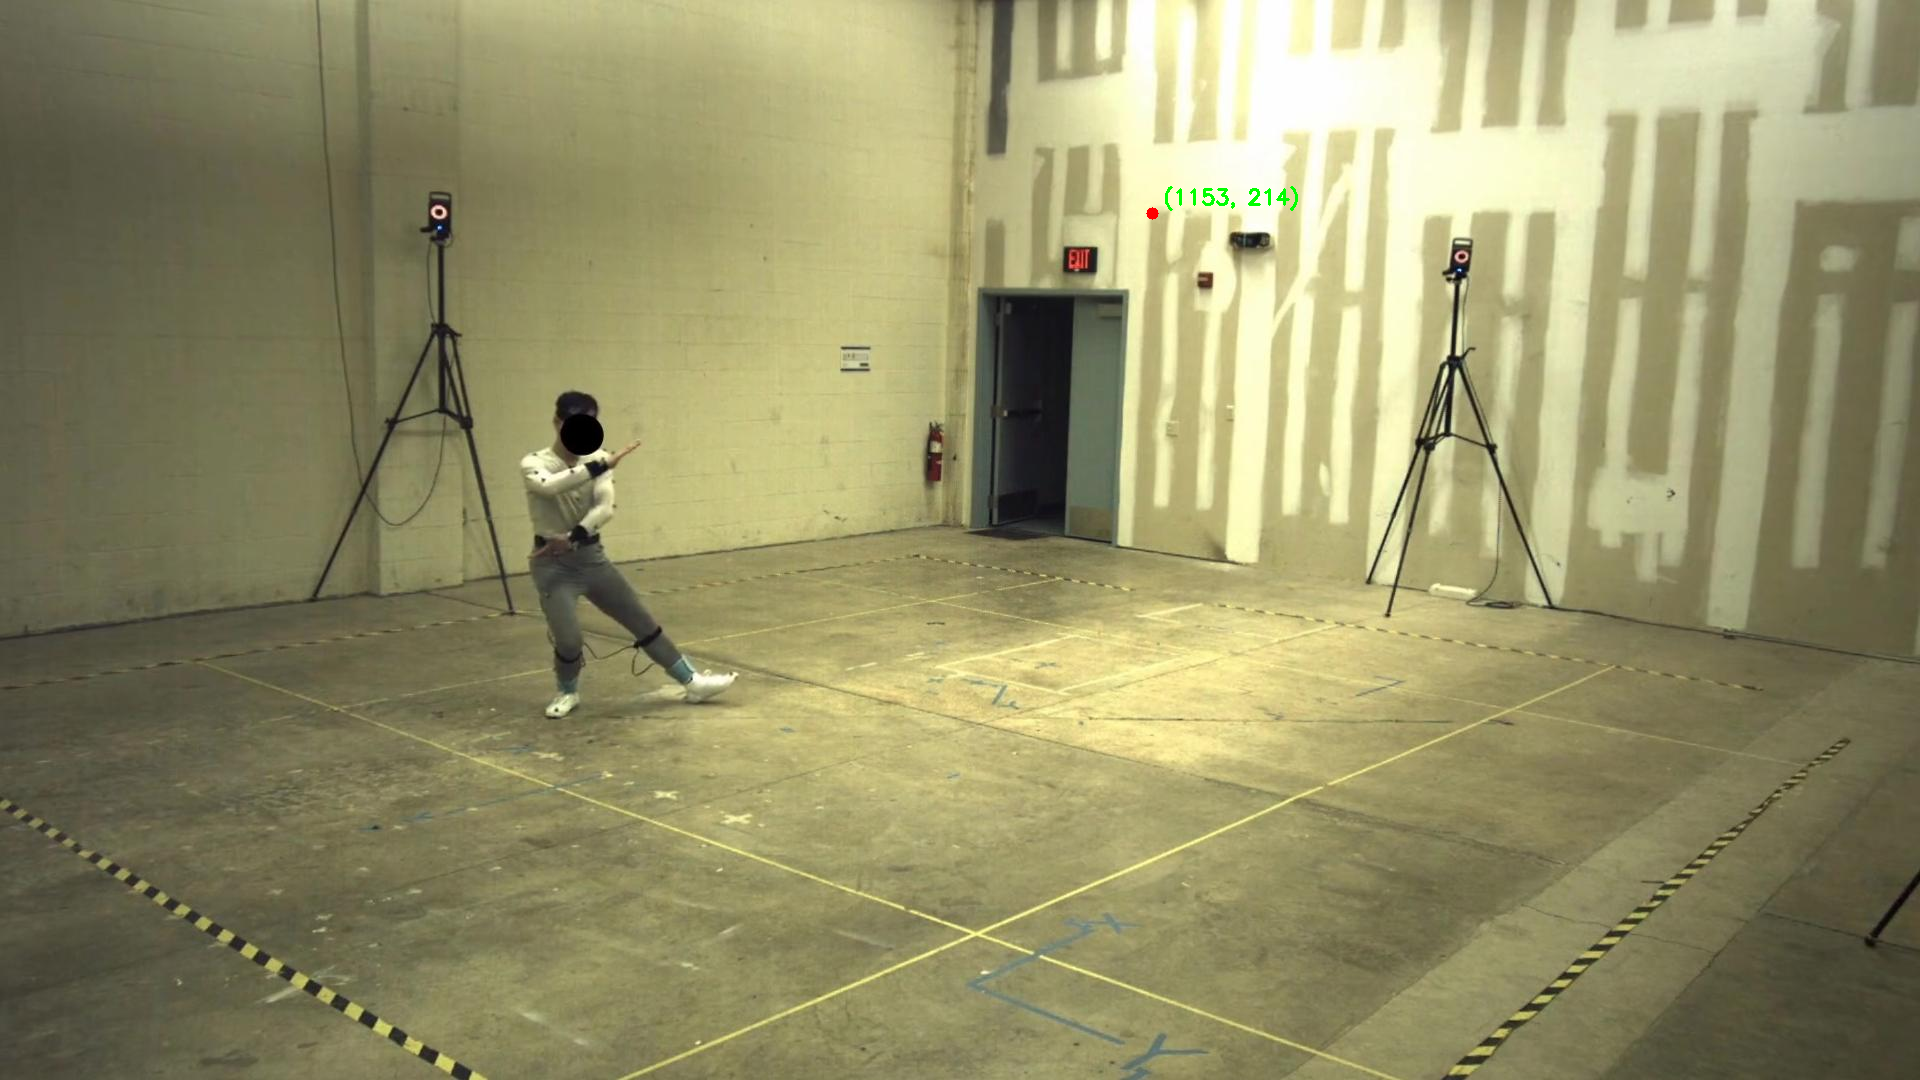
\includegraphics[width=0.32\linewidth]{img1_pts1.png}
    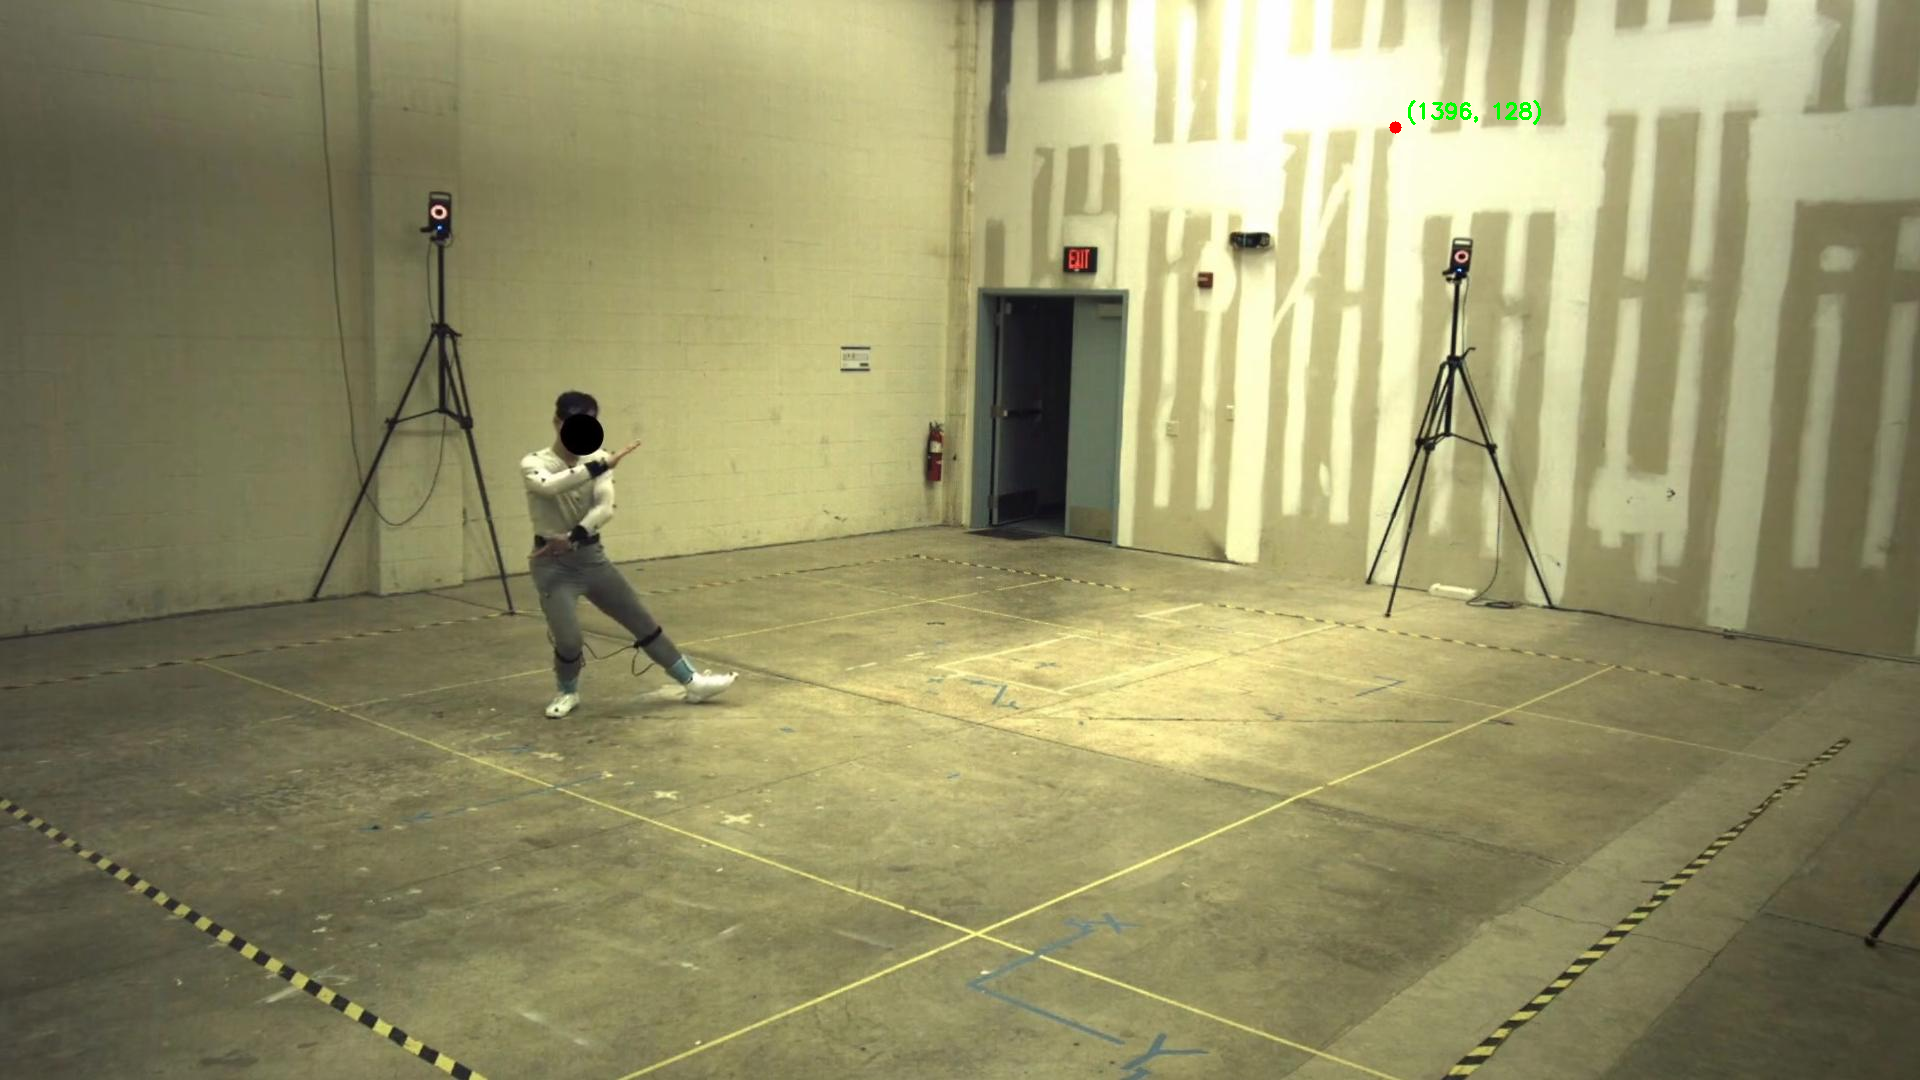
\includegraphics[width=0.32\linewidth]{img1_pts2.png}
    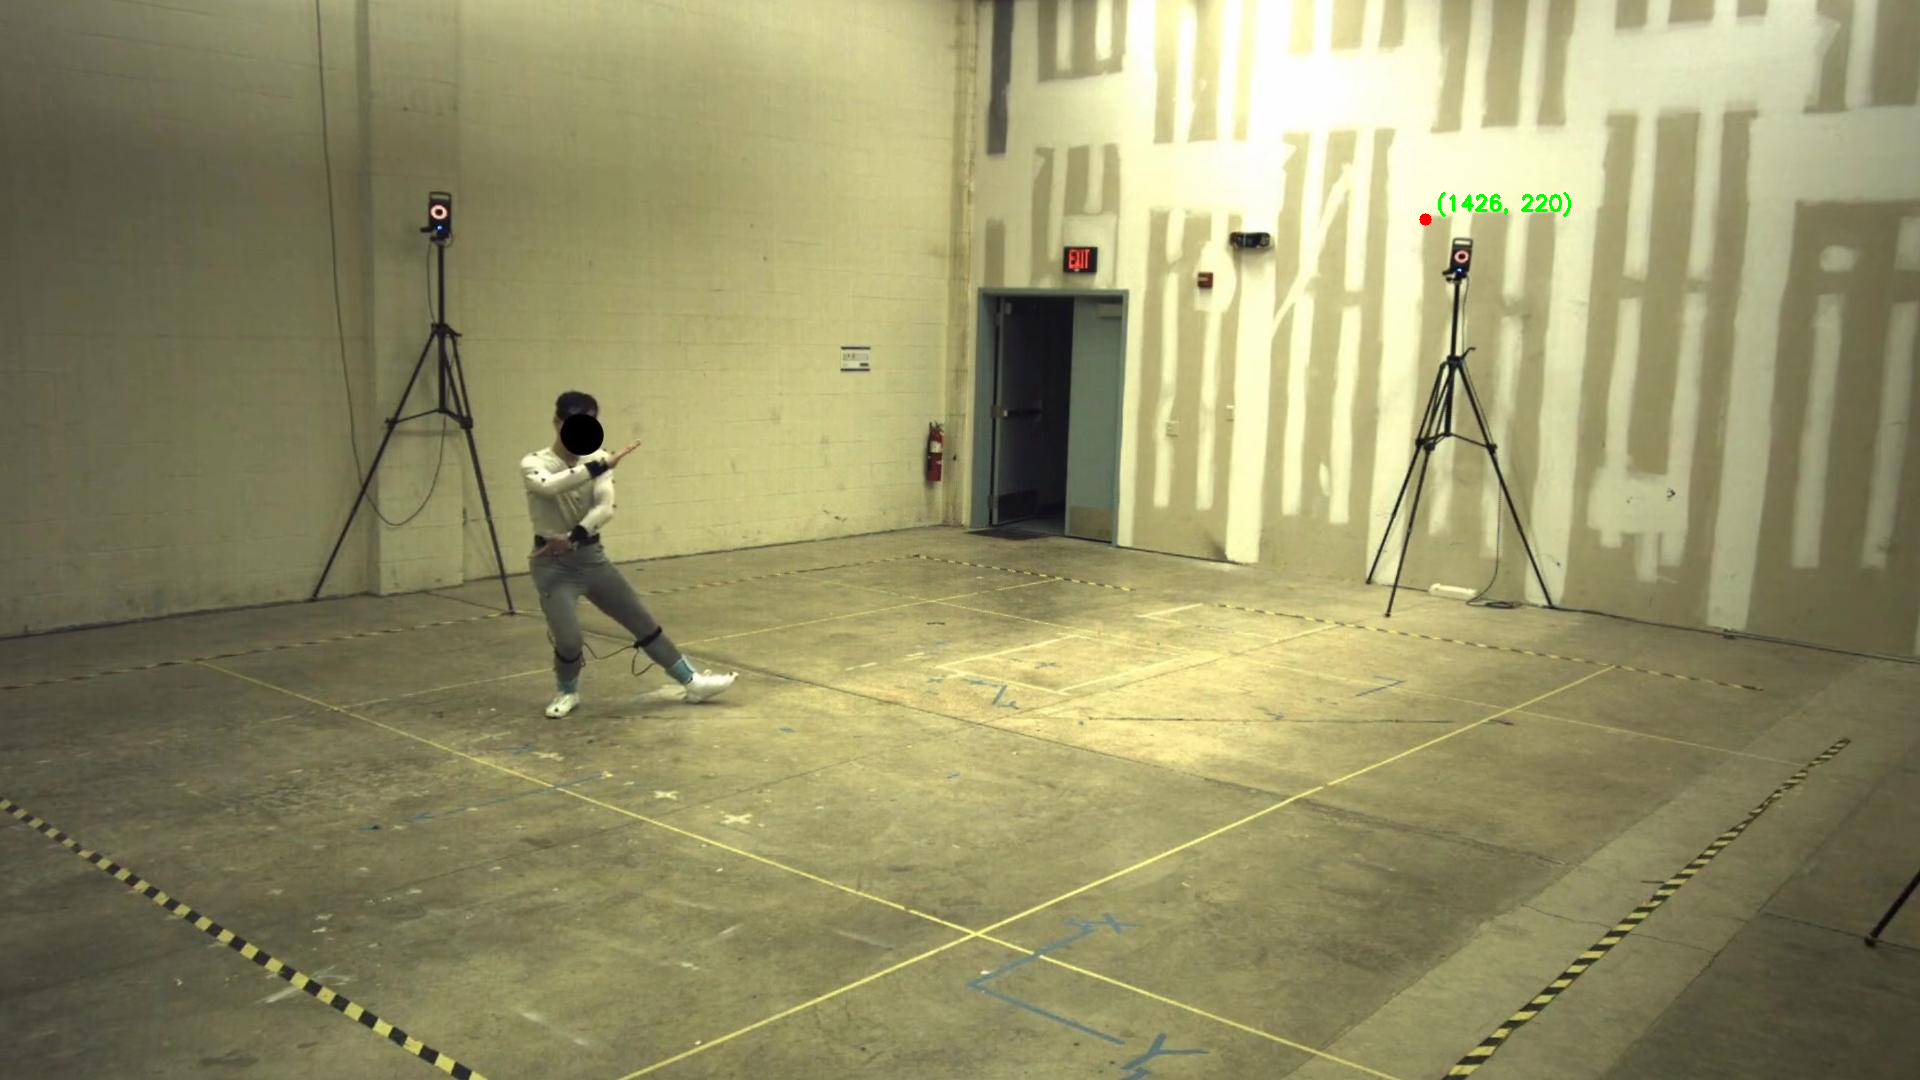
\includegraphics[width=0.32\linewidth]{img1_pts3.png}

    \medskip

    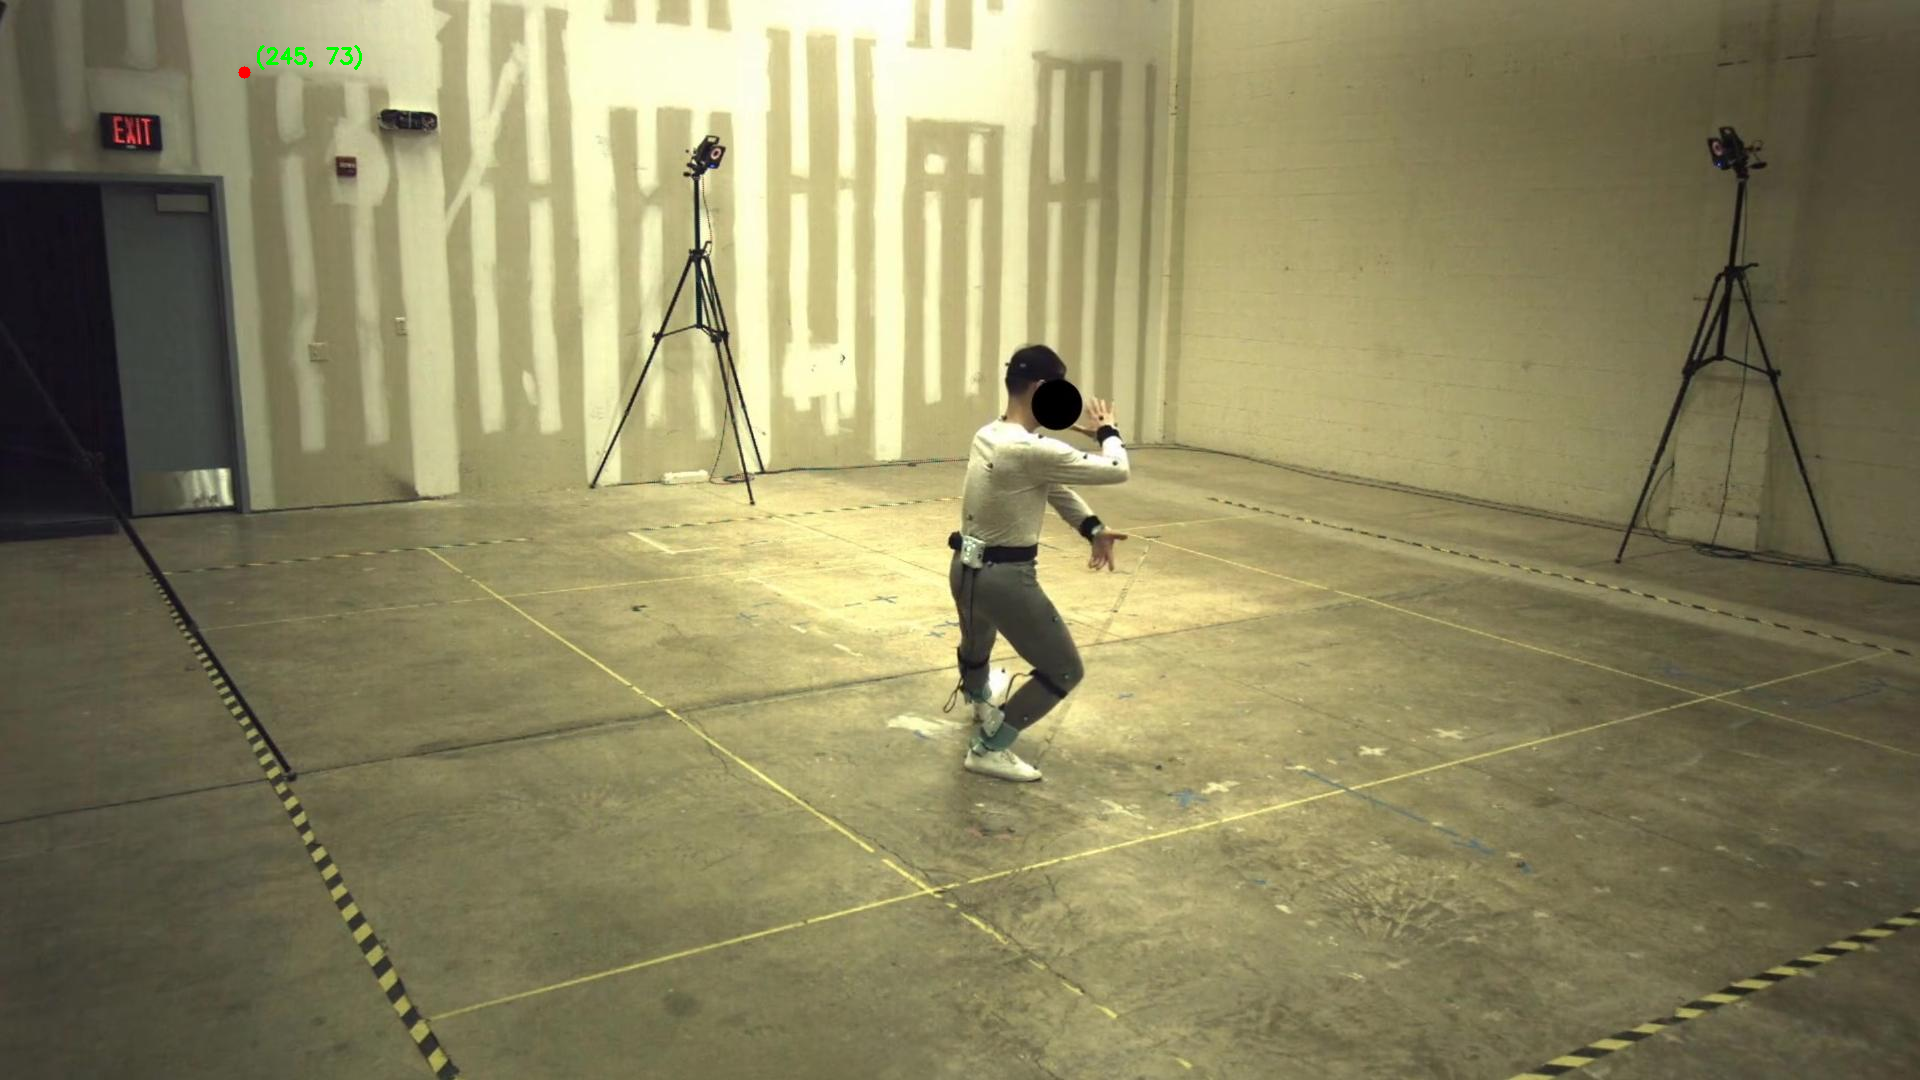
\includegraphics[width=0.32\linewidth]{img2_pts1.png}
    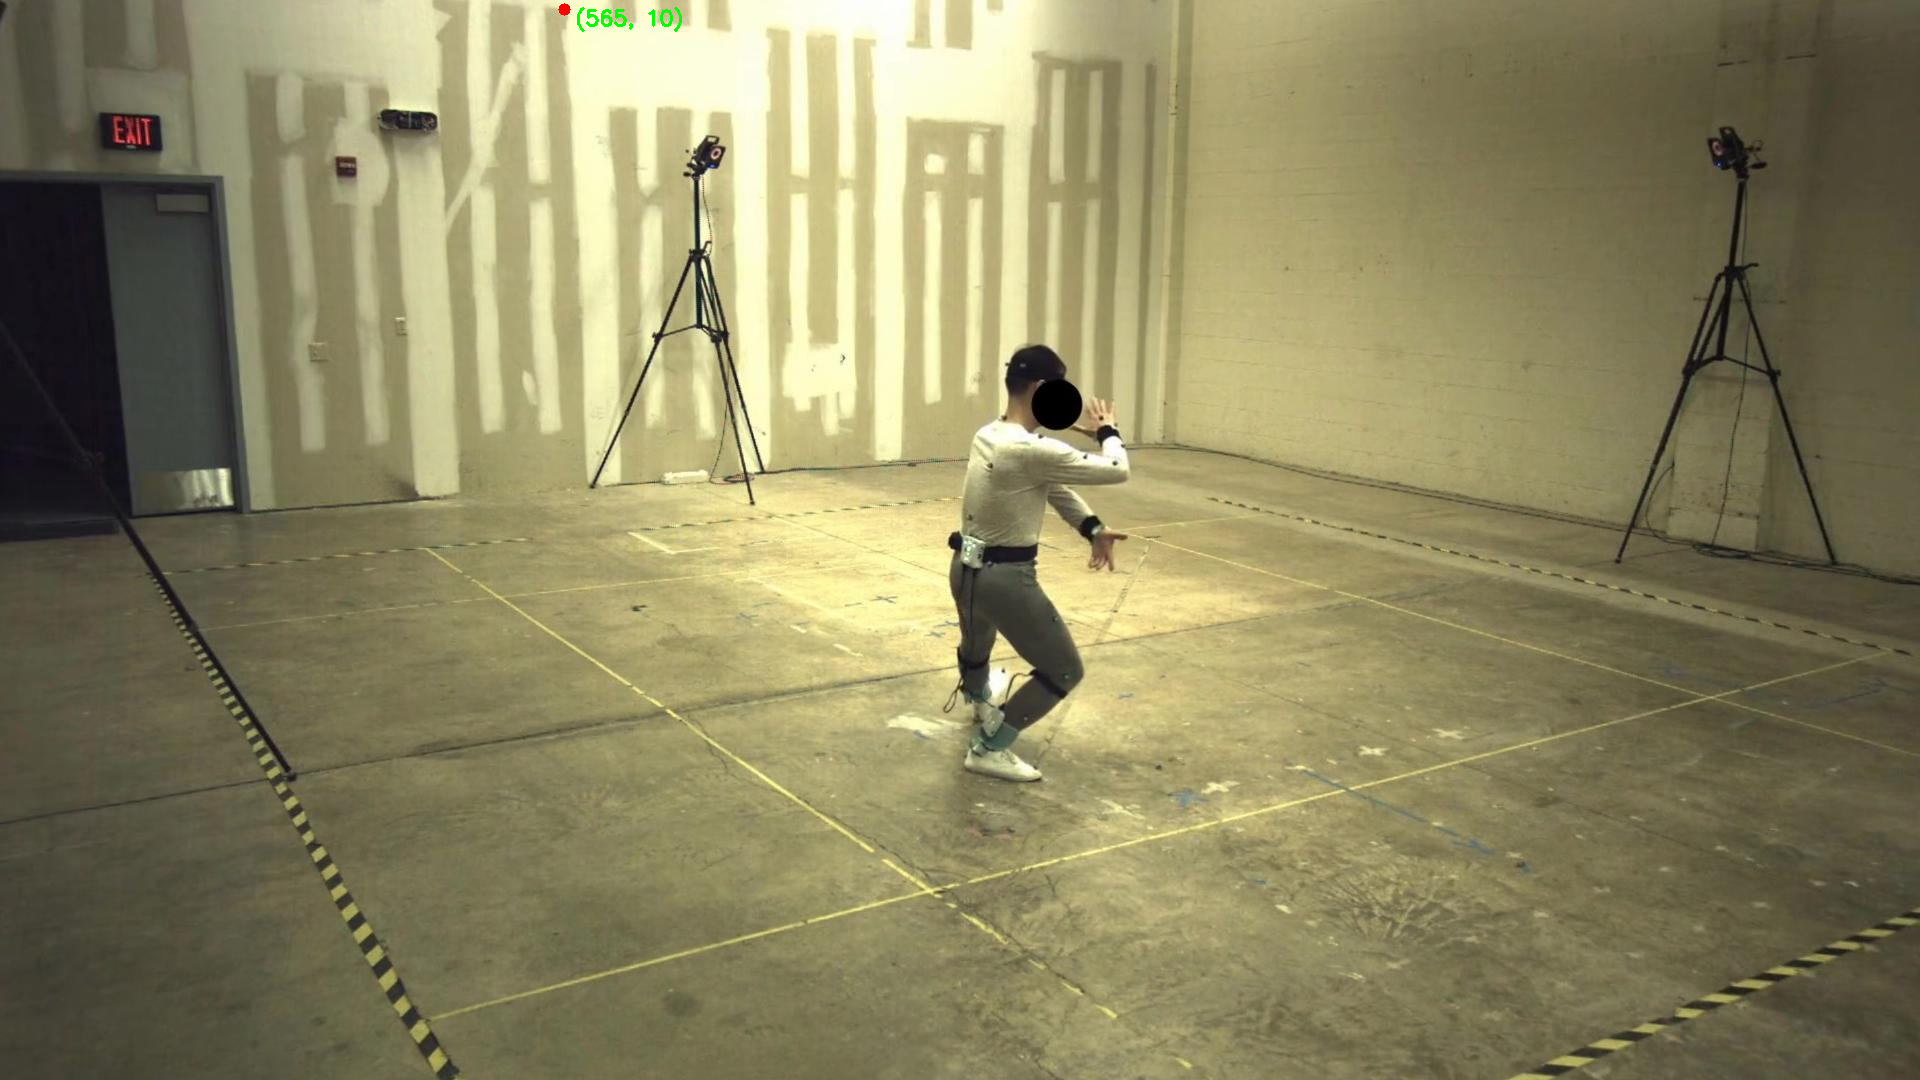
\includegraphics[width=0.32\linewidth]{img2_pts2.png}
    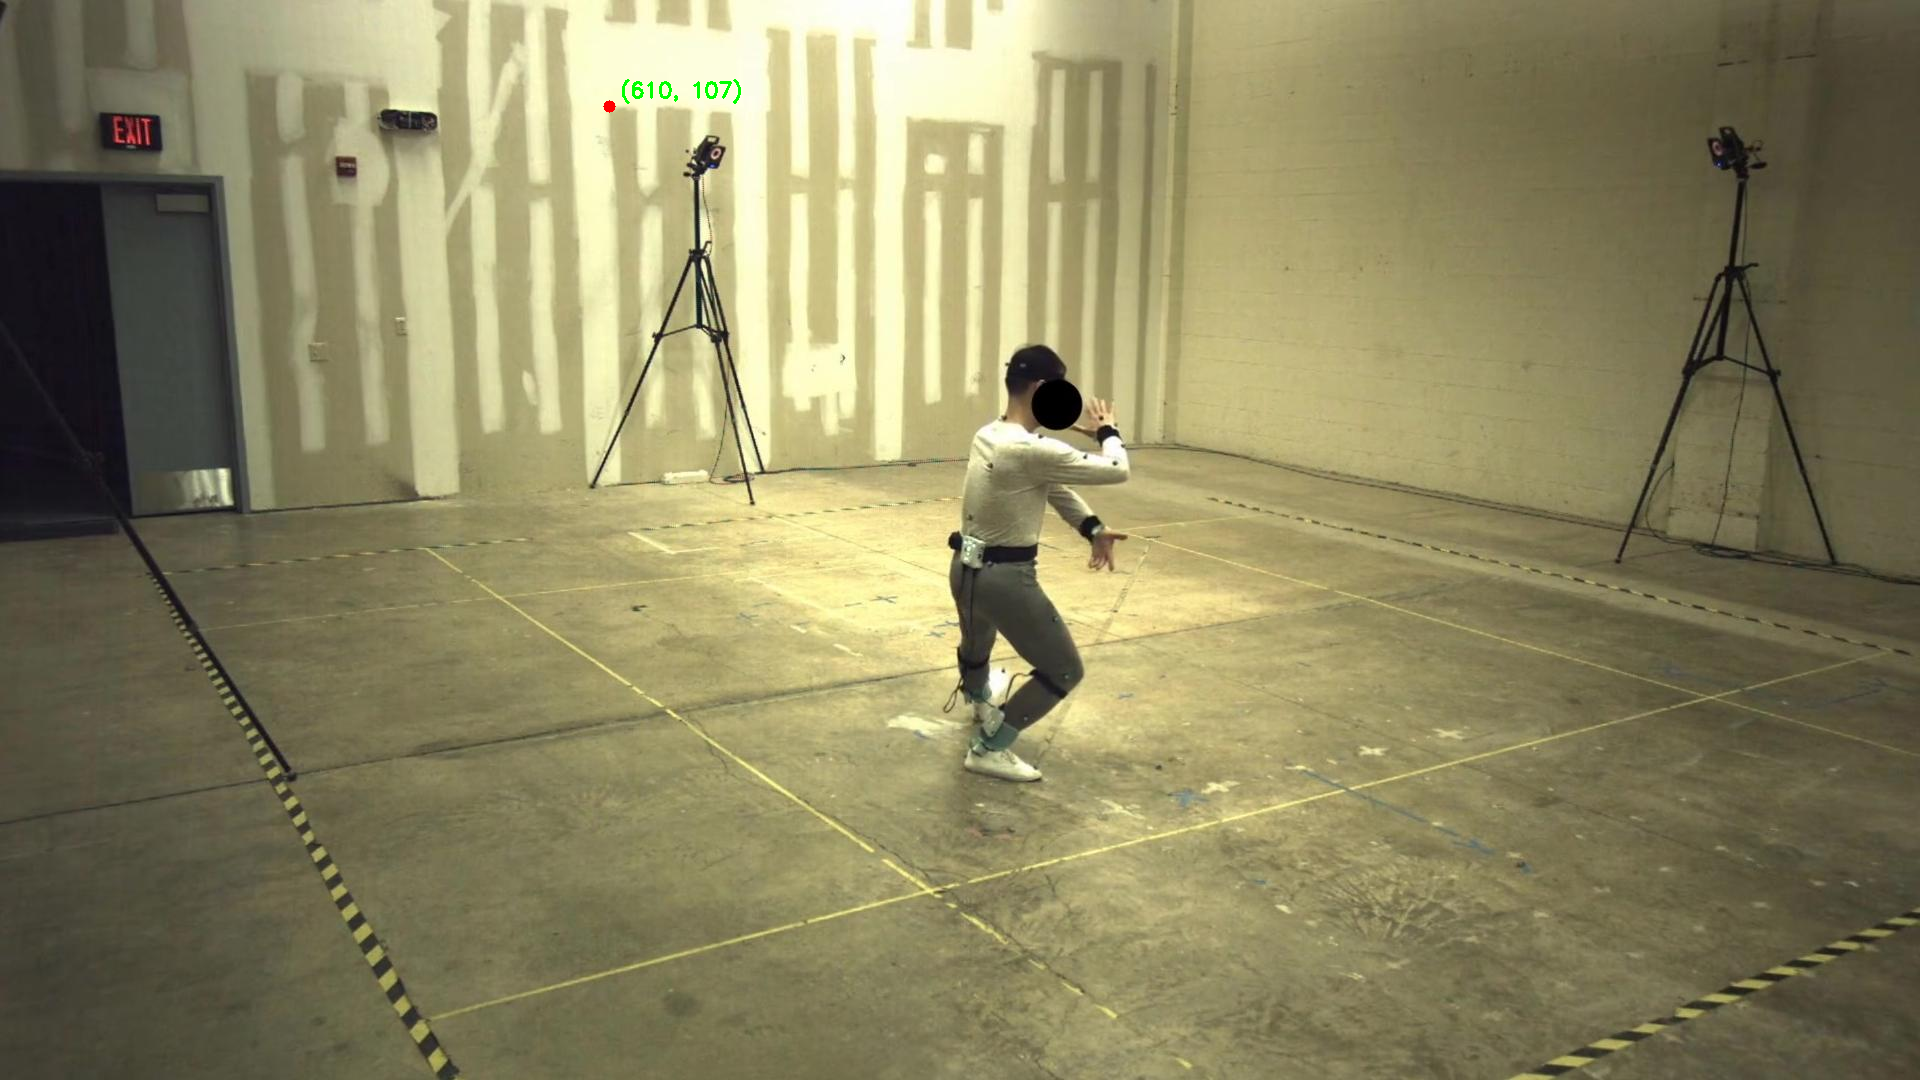
\includegraphics[width=0.32\linewidth]{img2_pts3.png}
    \caption{Wall points clicked in image 1 (top row) and image 2 (bottom row).}
    \label{fig:task3-4-wall}
\end{figure}

the fitted wall plane is:
\[
Wall\ plane:  0.00498018623082 x +0.999408337944 y +0.0340319231535 z +5443.91062186 = 0
\]
which is approximately the vertical plane $Y \approx -5444$ mm.

\subsection*{Height of the Door}
we clicked the top of the doorway in both images and triangulated the point. taking the floor as $Z=0$, the doorway si about \textbf{2034 mm} (2.03 m) tall.

\begin{figure}[H]
    \centering
    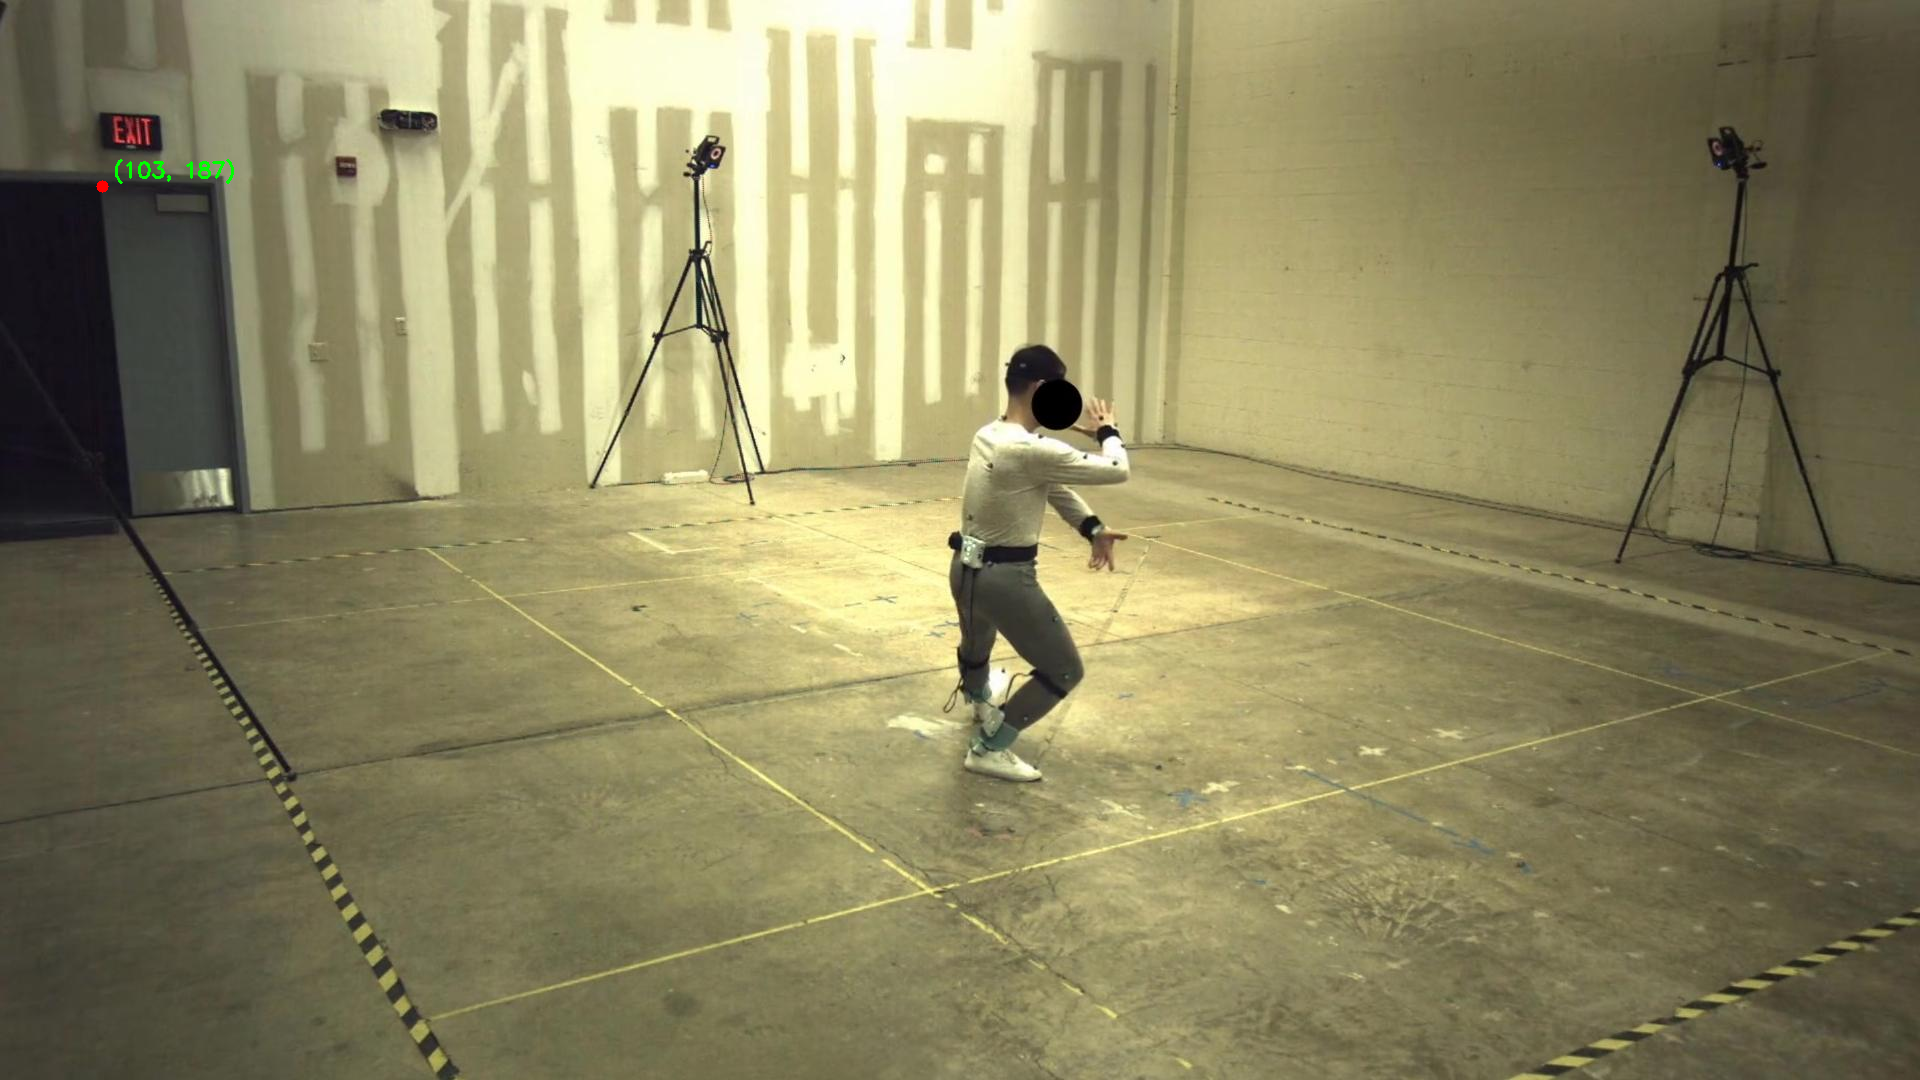
\includegraphics[width=0.48\linewidth]{1_door_pt.png}
    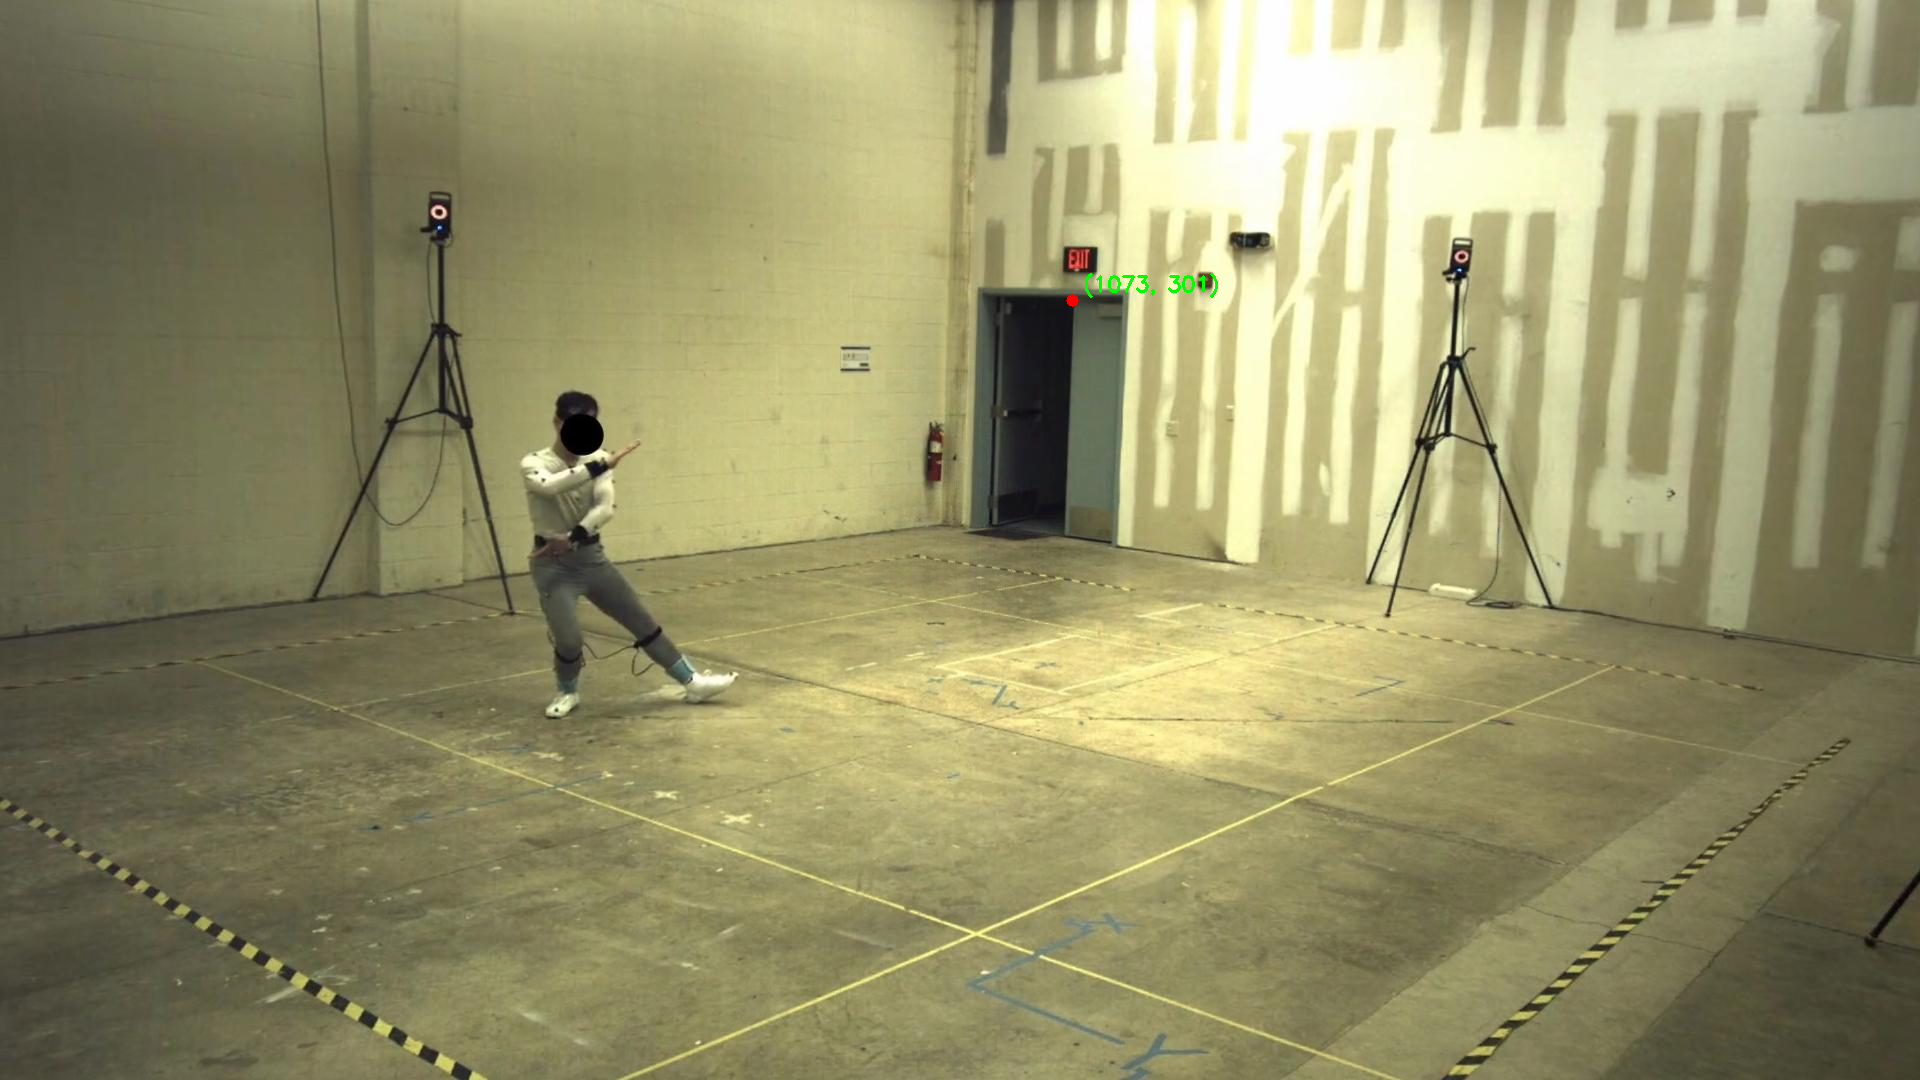
\includegraphics[width=0.48\linewidth]{2_door_pt.png}
    \caption{Doorway top point clicked in image 1 (left) and image 2 (right).}
    \label{fig:task3-4-door}
\end{figure}

\subsection*{Height of the Person}
We clicked the top of the person's head in both images and triangulated it. The head is about \textbf{1462 mm}. The person is in a lunge in this frame, so this below standing height. 

\begin{figure}[H]
    \centering
    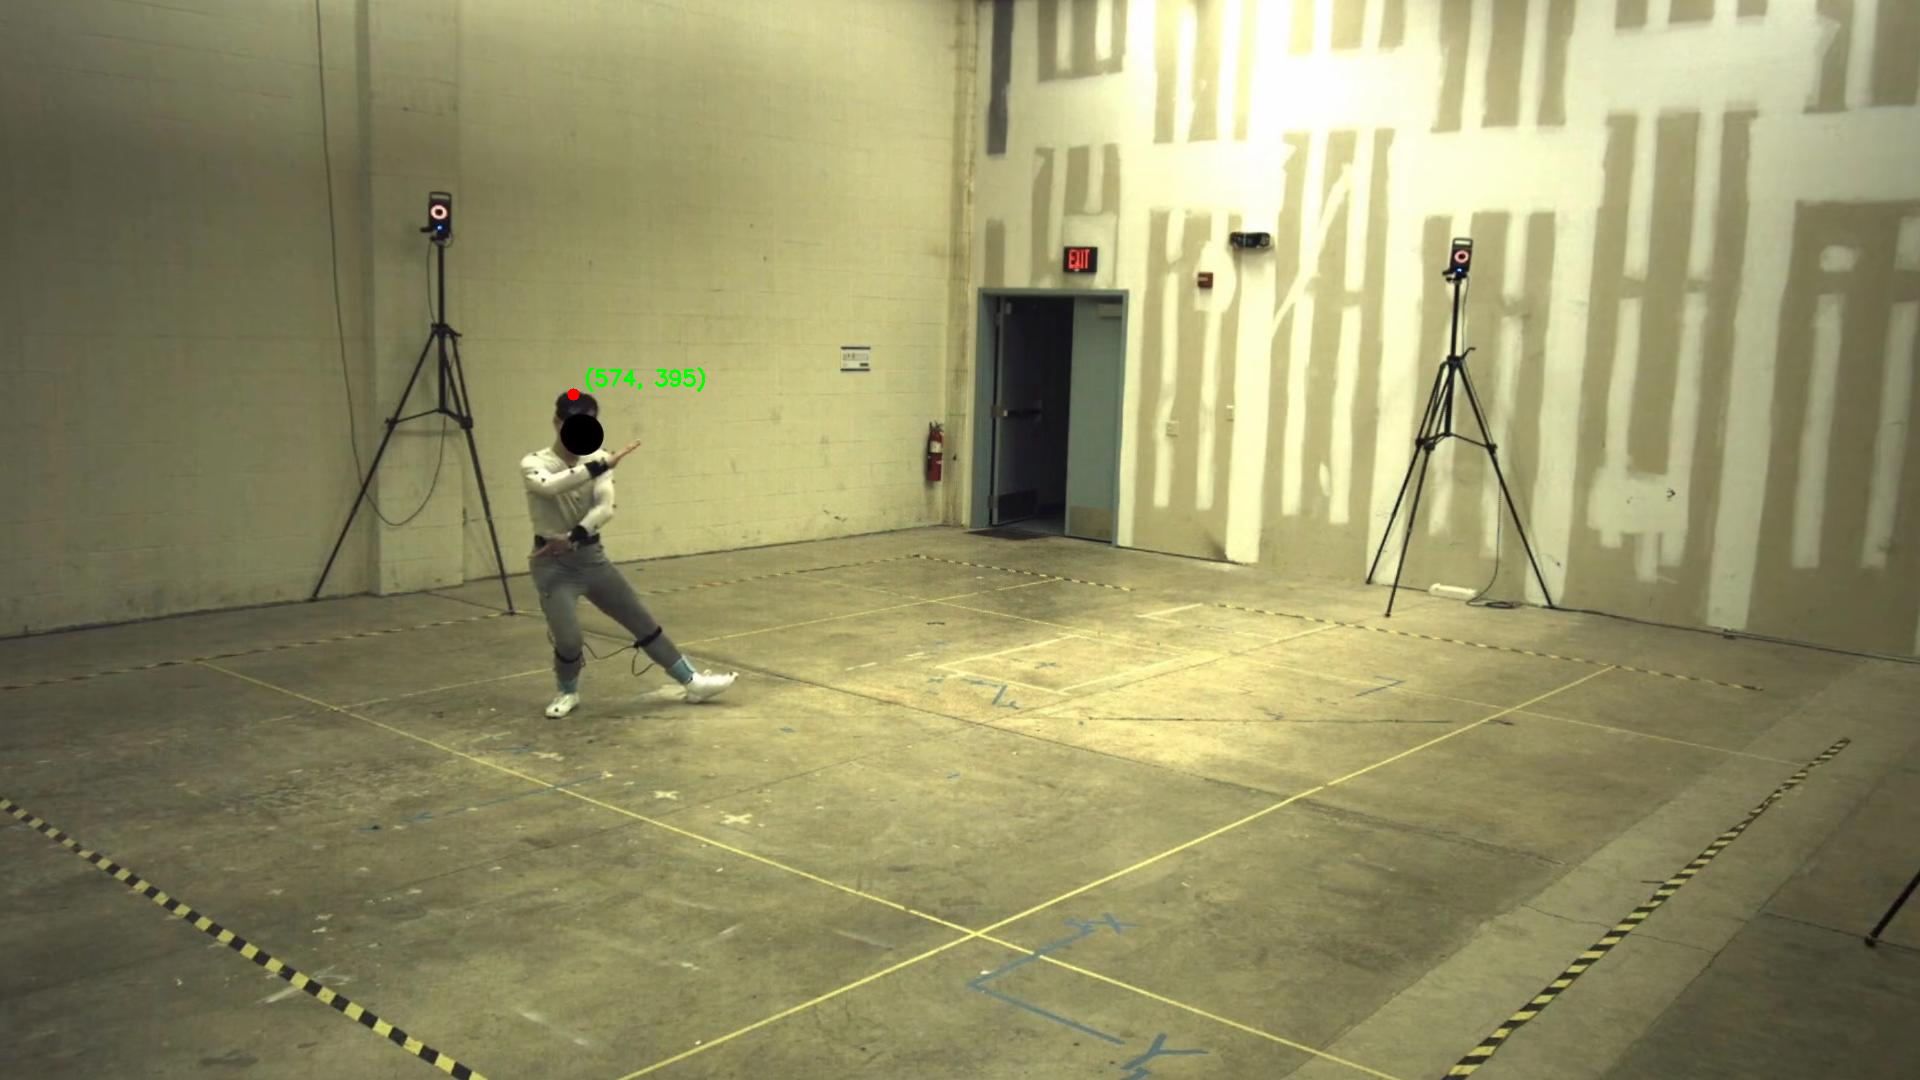
\includegraphics[width=0.48\linewidth]{1_person_pt.png}
    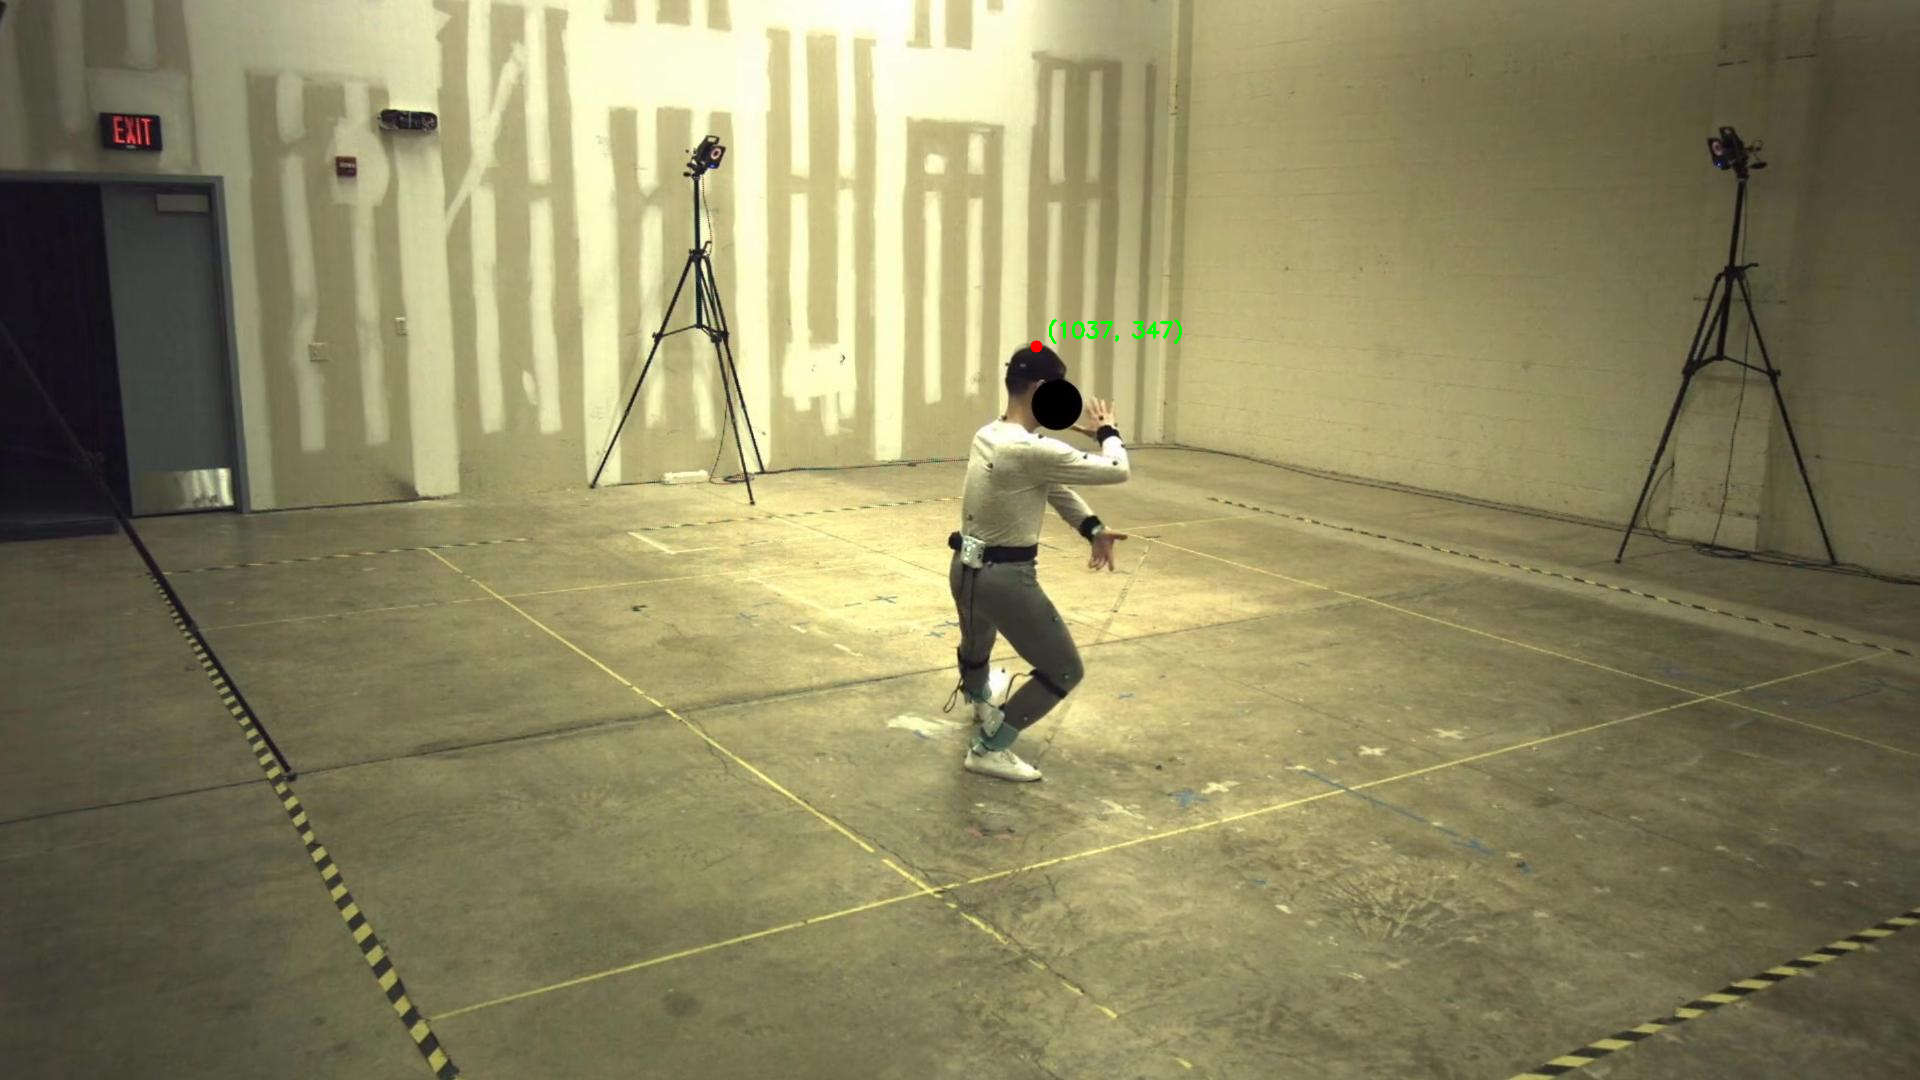
\includegraphics[width=0.48\linewidth]{2_person_pt.png}
    \caption{Top of the head clicked in image 1 (left) and image 2 (right).}
    \label{fig:task3-4-person}
\end{figure}

\subsection*{Camera Location}
We clicked the center of the camera of the camera on the tall tripod in both images and triangulated it. The location is shown to be about \textbf{$(-76,\ -4894,\ 2418)$ mm}. Its $Y$ value is within about half a meter of the wall plane, so the tripod stands near the striped wall, as described within the assignment.

\begin{figure}[H]
    \centering
    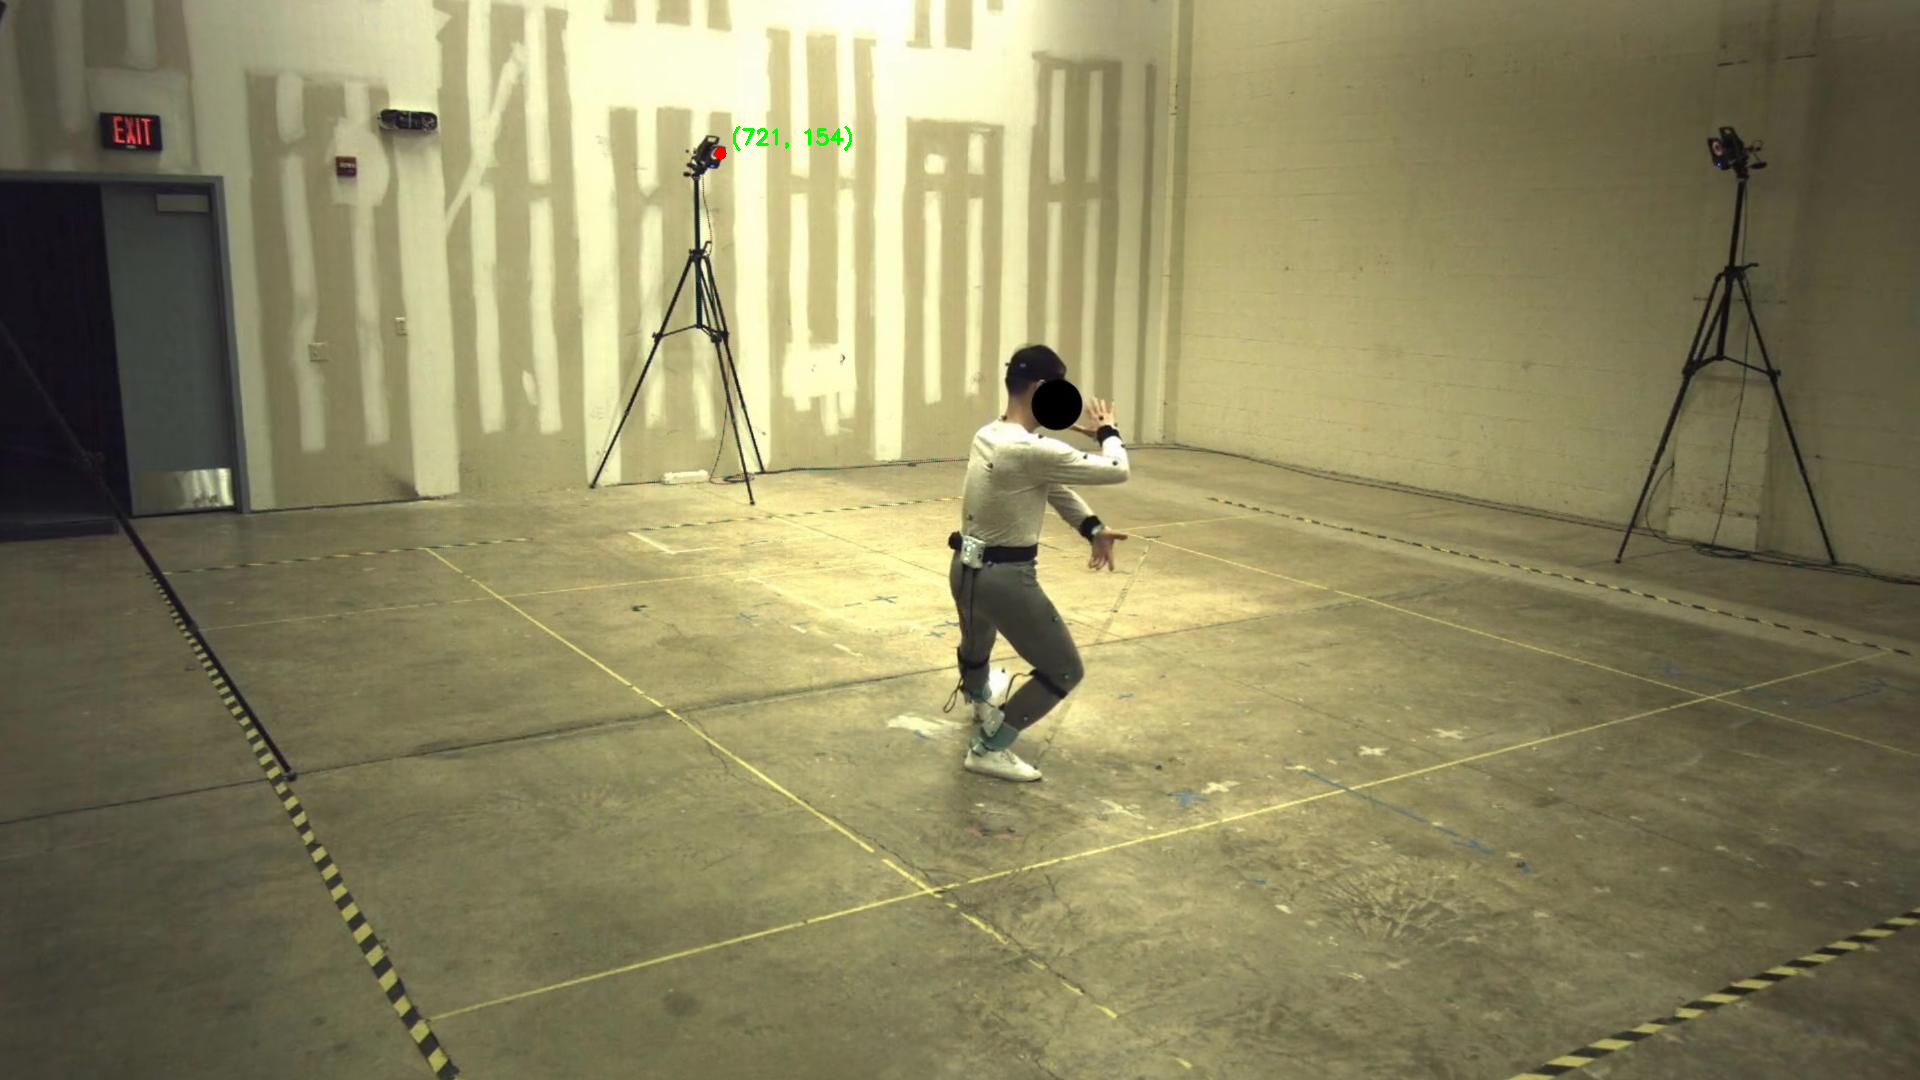
\includegraphics[width=0.48\linewidth]{1_cam_pt.png}
    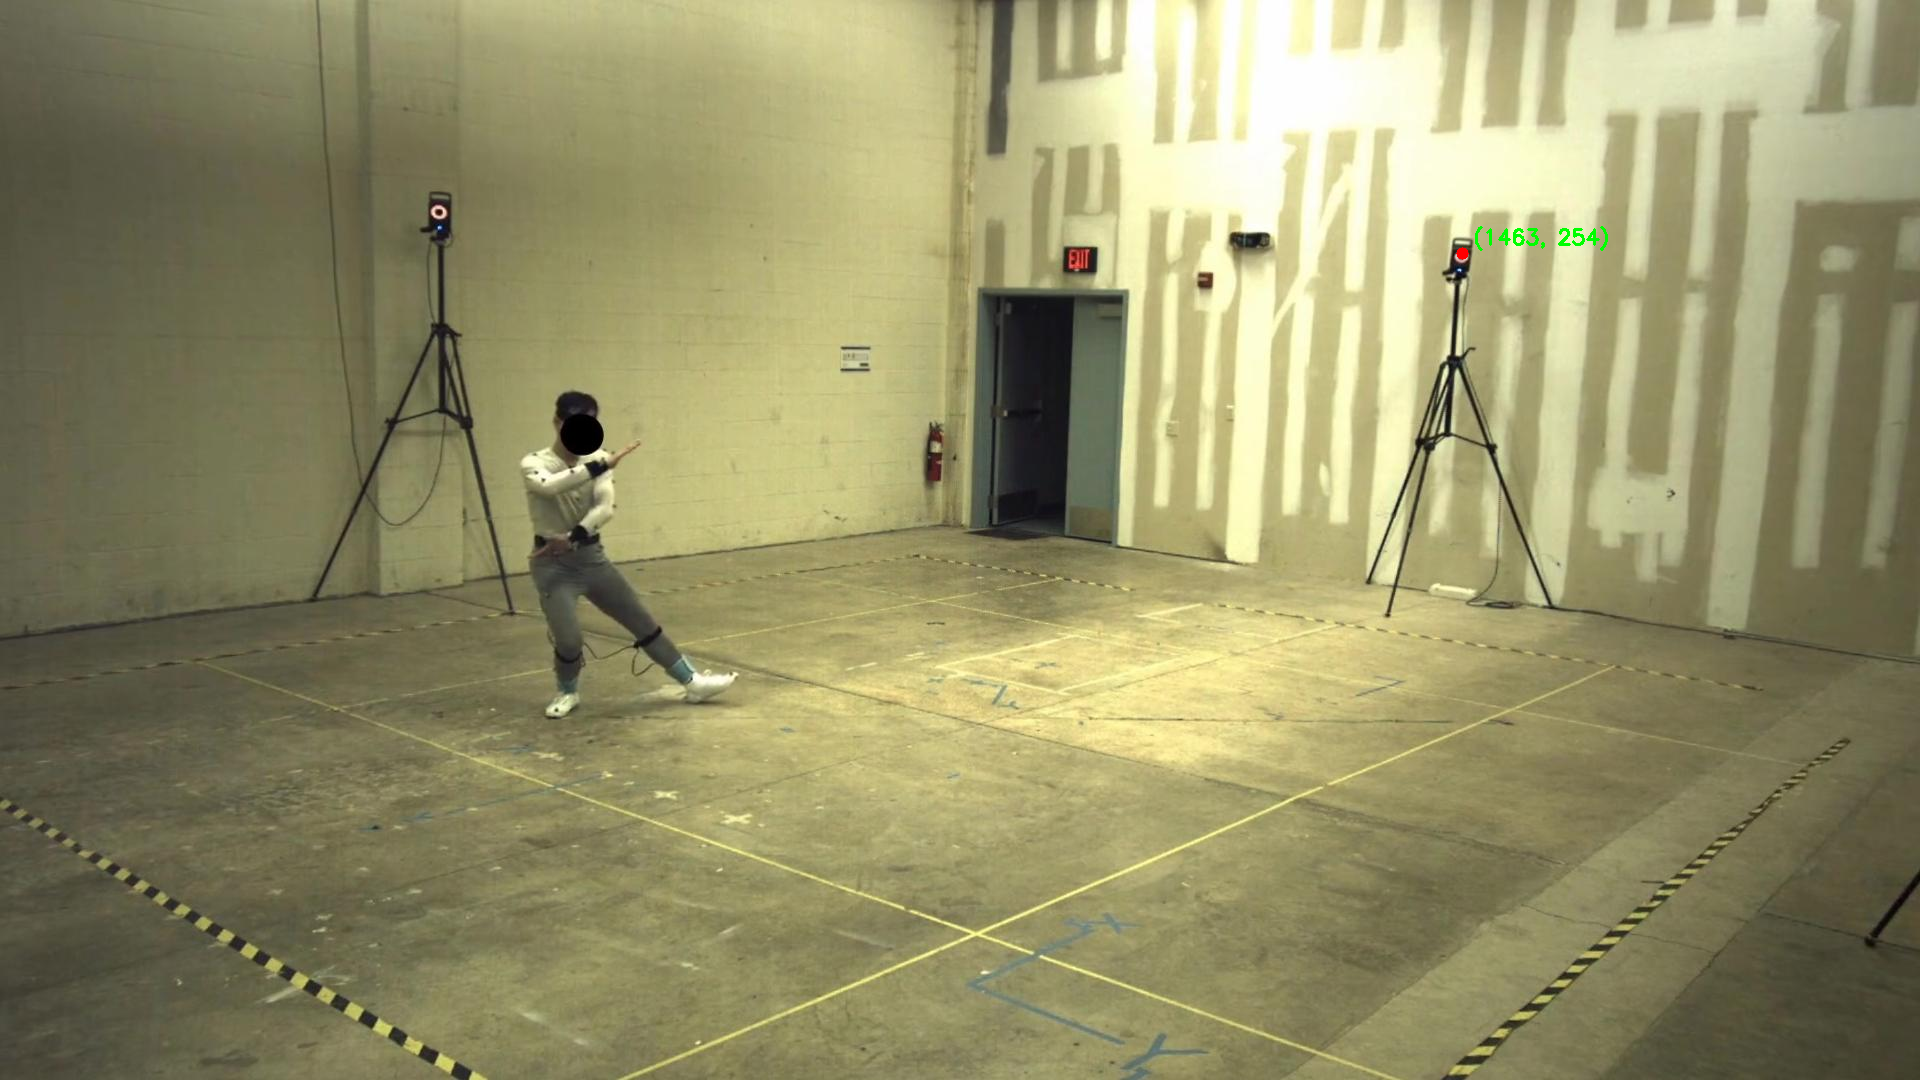
\includegraphics[width=0.48\linewidth]{2_cam_pt.png}
    \caption{Tripod camera center clicked in image 1 (left) and image 2 (right).}
    \label{fig:task3-4-camera}
\end{figure}

\tasksection{Task 3.5}{Fundamental Matrix from Camera Parameters}
\label{sec:task3-5}

\subsection*{Relative rotation and position of camera 2}
From Task 3.1, a world point $X$ becomes camera coordinates by $X_{cam,j}=R_j(X-C_j)$. Solving the camera 1 equation for $X$ gives $X = R_1^T X_{cam,1} + C_1$, since $R_1^{-1}=R_1^T$ for a rotation matrix. Substituting into the camera 2 equations gives:

\[
X_{cam,2} = R_2 R_1^T\, X_{cam,1} + R_2 (C_1 - C_2)
\]

\medskip

The relative rotation of camera 2 with respect to camera 1 is computed using the matric multiplication $X_{cam,1}$ above:
\[
R=R_2 R_1^T
\]

\medskip

The position of the camera 2 in camera 1's coordinate system is computed by the vector from camera 1 to camera 2 in world coordinates, rotated into camera 1's frame (the same transform that takes world points to camera 1):

\[
T = R_1 (C_2 - C_1)
\]

\subsection*{Essential and Fundamental Matrices}
Let $S$ be the skew-symmetric matrix of $T = [t_1, t_2, t_3]$, so that $Sp = T\times p$

\[
S = \begin{bmatrix}
    0 & -t_3 & t_2 \\ t_3 & 0 & -t_1 \\ -t_2 & t_1 & 0
\end{bmatrix}
\]

\medskip

The essential matrix is $E = R\cdot\,S$. It relates points in normalized camera coordinates. To work in pixel coordinates we use $x = \texttt{Kmat}\cdot\ x_{norm}$, which gives us:

\[
F = \texttt{Kmat}_2^{-T}\cdot\ E\cdot\ \texttt{Kmat}_1^{-1},
\qquad
x_2^T F x_1 = 0
\]

where $x_1, x_2$ are homogeneous pixels points in images 1 and 2. The matrix is scaled to unit norm, which does not change the epipolar lines. The result is:

\[
F \approx
\begin{bmatrix}
-6.32\times10^{-8} & 1.29\times10^{-6} & -3.97\times10^{-4} \\
 1.52\times10^{-6} & 2.15\times10^{-7} &  1.32\times10^{-3} \\
-1.97\times10^{-4} & -4.46\times10^{-3} & 1.0000
\end{bmatrix}.
\]

\subsection*{Epipolar Lines}
A point $x_1$ in images 1 maps to the line $l_2 = F x_1$ in image 2, and a point $x_2$ in image 2 maps to the line $l_1 = F^T x_2$ in image 1. Figure~\ref{fig:tasks3-5} draws these lines for the ten matched points that were clicked by hand for Task 3.6, with each point and its line in the same color. 

\begin{figure}[H]
    \centering
    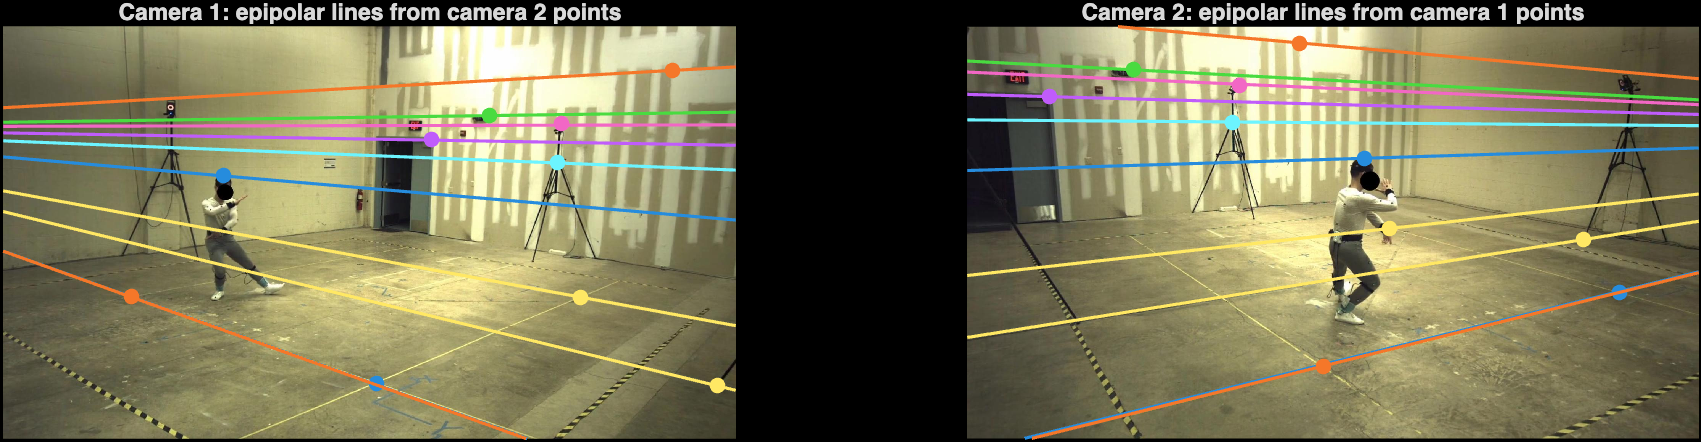
\includegraphics[width=\linewidth]{Camera-parameter_epipolar.png}
    \caption{Epipolar lines from the calibration-based F for the clicked matched points.}
    \label{fig:tasks3-5}
\end{figure}

In both directions, each point lies on, or is very close to its epipolar line. The lines in each images are nearly horizontal and converge towards a common point, the epipolar, as expected for two cameras at similar heights on opposite sides of the room. Two lines near the bottom of image 2 almost coincide because their points lie close together on the floor. 

Quantitatively, the symmetric epipolar distance of this $F$ over all the 39 projected point matches is $9\times10^{-27}$ pixels$^2$, which is zero to floating-point precision. 

\tasksection{Task 3.6}{Fundamental Matrix from Point Correspondences}
\label{sec:task3-6}
\subsection*{Eight-Point Algorithm Demo}

First step of Task 3.6 is running the eight-point algorithm demo provided by the instructor (\texttt{eightpointprecanned}) on the Old Main images. It prints the following fundamental matrix:

\[
F_{\text{demo}} =
\begin{bmatrix}
-0.0109502 & -0.0163594 & 41.2715 \\
0.00877517 & 0.014063   & 7.56831 \\
-5.67981   & -9.36867   & -16253.4
\end{bmatrix}.
\]

This matrix is not scaled to unit norm, so its entries ar much larger than those of our $F$. The scale doesn't change the epipolar lines. Figures~\ref{fig:demo1} and ~\ref{fig:demo2} show the epipolar lines drawn by the demo. 

\begin{figure}[H]
  \centering
  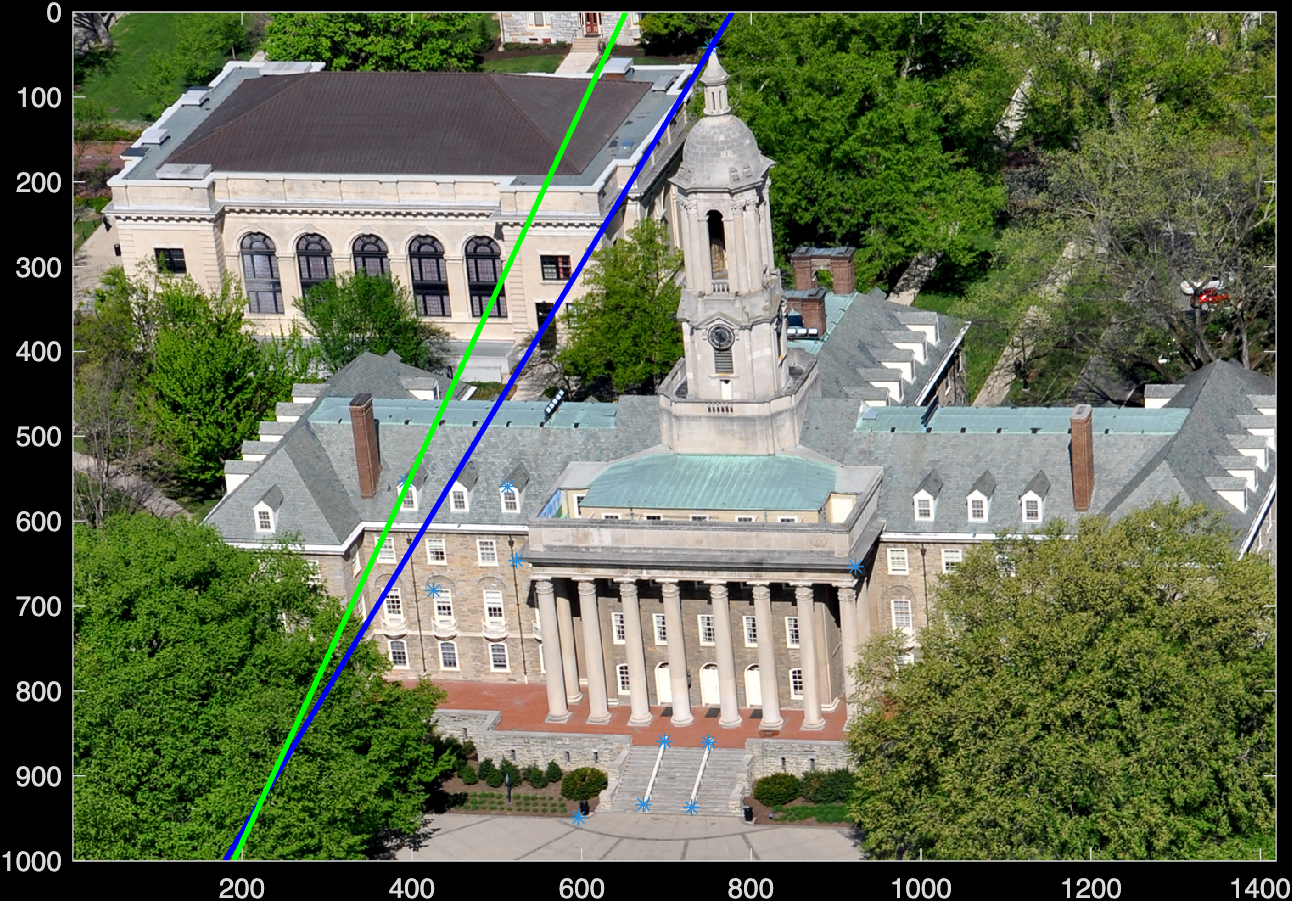
\includegraphics[width=0.8\textwidth]{demo_fig1.png}
  \caption{Epipolar lines from the demo, first image.}
  \label{fig:demo1}
\end{figure}

\begin{figure}[H]
  \centering
  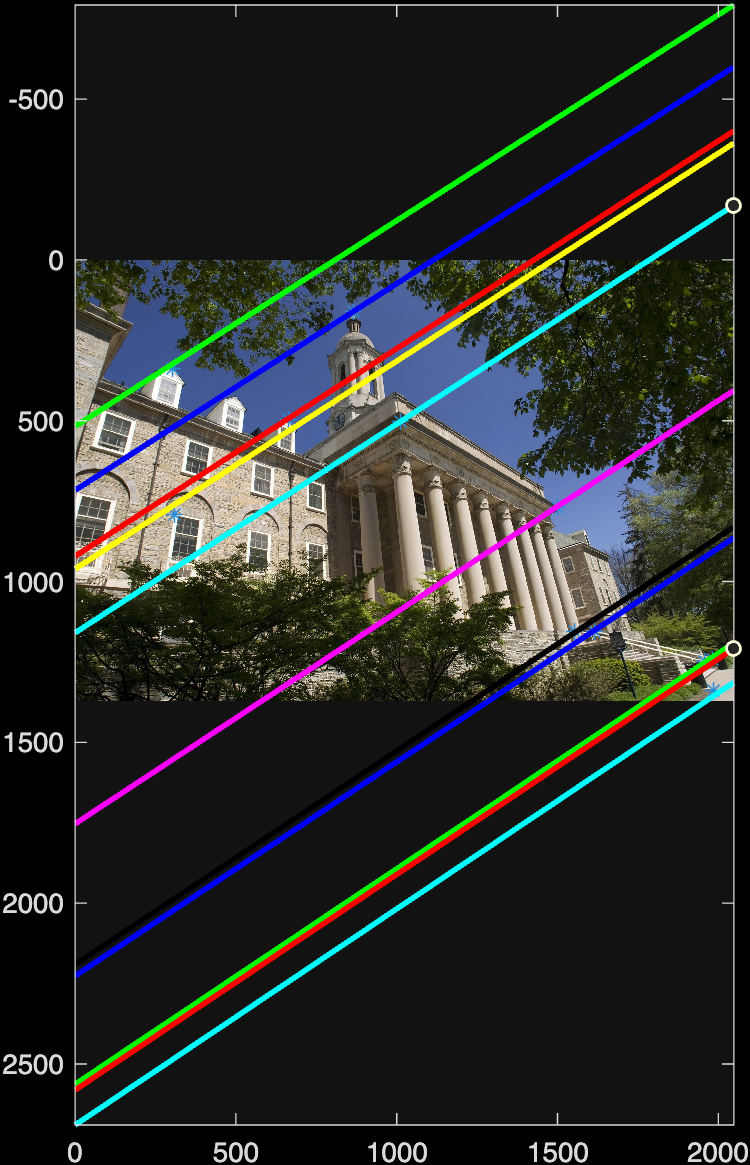
\includegraphics[width=0.5\textwidth]{demo_fig2.png}
  \caption{Epipolar lines from the demo, second image.}
  \label{fig:demo2}
\end{figure}


\subsection*{Method}

We estimated $F$ from ten matched points selected by hand in the two images. The eight-point algorithm needs at least eight correspondences, but with exactly eight points the estimate had a huge error, so we added two more points to reduce the error. With more than eight points the system is overdetermined and is solved in the least-squares sense by the SVD. The pixel coordinates were saved in the folder \texttt{eight\_points} and are set in \texttt{main}. The function follows the eight-point algorithm from the course lecture and demo:

\begin{enumerate}
    \item \textbf{Normalize:} The points of each image are shifted to zero
          mean and divided by their standard deviation in $x$ and $y$
          (Hartley's preconditioning). This is a matrix $T_j$ with
          $\hat{x}=T_jx$, and it keeps the linear system well
          conditioned.
    \item \textbf{Build the system:} Each match gives one row of the
          $10\times9$ matrix $A$ from the constraint $x_2^TFx_1=0$.
    \item \textbf{Solve:} The unit vector $f$ minimizing $\|Af\|$ is the
          last column of $V$ in $A=U\Sigma V^T$ (equivalently, the
          eigenvector of $A^TA$ with the smallest eigenvalue). It is
          reshaped into a $3\times3$ matrix.
    \item \textbf{Enforce rank 2:} A true fundamental matrix is singular,
          so we take the SVD of $F$, set the smallest singular value to
          zero, and recompose.
    \item \textbf{Denormalize:} $F \leftarrow T_2^T F\, T_1$, which is
          equivalent to the lecture's $F=(T')^{-1}F_nT$, then scale to
          unit norm.
\end{enumerate}

Recommended in the class lecture, the ten points are chosen to span 3D scene rather than lying on a single plane such as the floor. 

\subsection*{Result}
The returned fundamental matrix is: 

\[
F \approx
\begin{bmatrix}
-5.62\times10^{-8} & 1.19\times10^{-6} & -3.73\times10^{-4} \\
 1.52\times10^{-6} & 3.36\times10^{-7} &  1.16\times10^{-3} \\
-2.19\times10^{-4} & -4.31\times10^{-3} & 1.0000
\end{bmatrix}.
\]

Figure~\ref{fig:task3-6} shows the epipolar lines for the ten points in both directions, using $l_2=Fx_1$ in images 2 and $l_1=F^Tx_2$ in image 1.

\begin{figure}[H]
    \centering
    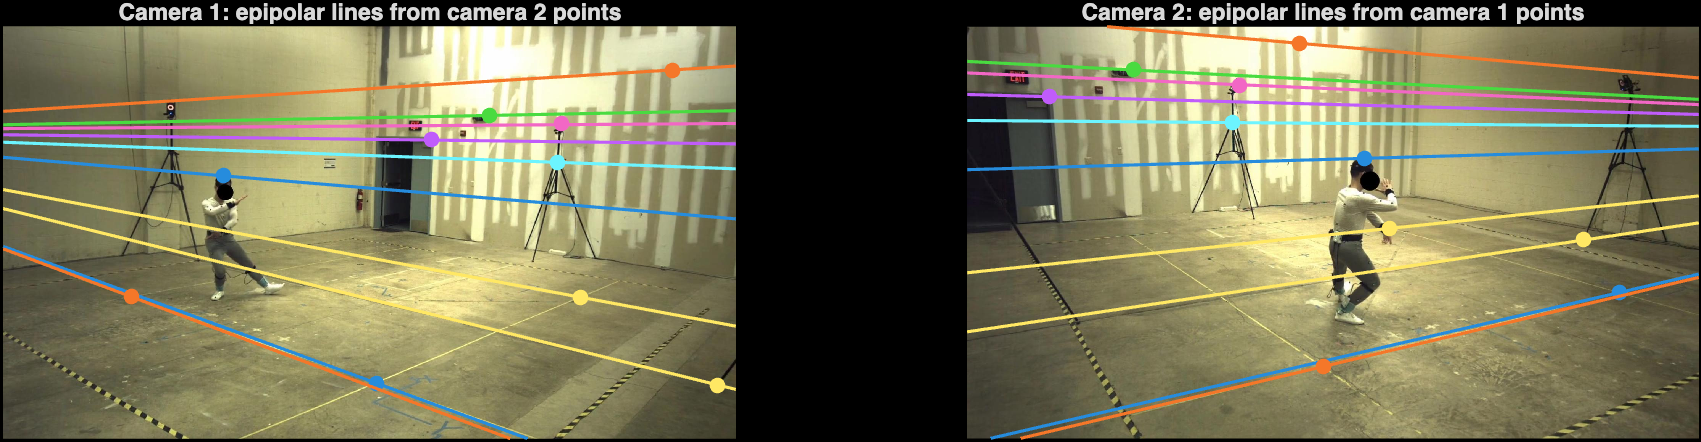
\includegraphics[width=\linewidth]{Eight-point_epipolar.png}
    \caption{Epipolar lines from the eight-point algorithm’s $F$ (ten points)}
    \label{fig:task3-6}
\end{figure}

This epipolar geometry looks reasonable as each point lies close to its epipolar line in both images, the lines ar nearly horizontal and coverage toward a common epipolar, and the pattern closely resembles the one from the calibration-based $F$ in Task 3.5. The ten-point result is slightly less accurate by a few lines, such as the blue and orange pair near the bottom which are visibly offset from their points. This is expected because the points were clicked by hand and the estimate uses only ten correspondences. Task 3.7 quantifies the difference.


\tasksection{Task 3.7}{Fundamental Matrix Evaluation}
\label{sec:task3-7}
\subsection*{Method}
To evaluate an estimated fundamental matrix quantitatively, we can use the symmetric epipolar distance (SED) on the 39 accurate point matches generated in Task 3.2. For a match $x_1=(x_1,y_1)$ in image 1 and $x_2=(x_2,y_2)$ in image 2, we computed:

\begin{enumerate}
    \item the epipolar line in image 2, $l_2 = F\tilde{x}_1 = (a,b,c)$,
          and the squared distance of $x_2$ to it;
    \item the epipolar line in image 1, $l_1 = F^T\tilde{x}_2 = (a,b,c)$,
          and the squared distance of $x_1$ to it.
\end{enumerate}

For a line $(a,b,c)$ and a point $(x,y)$, the squared geometric distance is:

\[
d^2 = \frac{(ax+by+c)^2}{a^2+b^2}.
\]

Dividing by $a^2+b^2$ is required to obtain a true Euclidean distance in pixel units. Without it the value would be an algebraic quantity with no physical meaning. The SED is the mean of all these squared distances, over both images and all 39 matches. The computation is implemented in the function \texttt{calculate\_SED}, which is called by \texttt{task3\_7} once for each fundamental matrix, using the same 39 matches for both. 

\subsection*{Results}

\begin{center}
\begin{tabular}{lc}
\toprule
Fundamental matrix & SED (pixel$^2$) \\
\midrule
Calibration-based, Task 3.5 & $8.96\times10^{-27}$ \\
Eight-point algorithm, Task 3.6 & $1.92$ \\
\bottomrule
\end{tabular}
\end{center}

The error of the calibration-based $F$ is smaller than that of the eight-point $F$, which is expected. It SED is zero to floating-point precision because it is computed exactly from the same camera parameters that generated the 39 matches. The eight-point $F$ has ane SED of 1.92 pixels${^2}$, i.e. An RMS distance of about 1.4 pixels, which comes from estimating $F$ from a small set of hand-clicked points.

In practice $\sqrt{\text{SED}}$ indicates how far from an epipolar line is expected for a true match. For the eight-point $F$ this is about 1.4 pixels, so a distance threshold of a few pixels would be reasonable for rejecting outlier matches, while the calibration-based $F$ would allow a very tight threshold. 

\tasksection{Extra Task 1}{Camera Geometry for Cropped Views}
\label{sec:extra-1}
\subsection*{Cropping and the modified $K$ matrices}

We cropped both images to a rectangle around the performer that contains all 39 projected mocap points. In full-image pixel coordinates, the crop for image 1 has top-left corner $(515,374)$ and bottom-right corner $(748,728)$, and the crop for image 2 has top-left corner $(935,328)$ and bottom-right corner $(1139,785)$.

Let $(x_1,y_1)$ be the top-left corner of a crop. a pixel $(x,y)$ in the full image maps to $(x',y')=(x-x_1+1,\ y-y_1+1)$ in the cropped image (the $+1$ is because that MATLAB pixel indices start at 1). In homogeneous form $\Tilde{x}'=T\tilde{x}$ with:

\[
T = \begin{bmatrix} 1 & 0 & 1-x_1 \\ 0 & 1 & 1-y_1 \\ 0 & 0 & 1 \end{bmatrix}.
\]

If a world point $w$ projects as $\tilde{x}=\texttt{Kmat}\,\texttt{Pmat}\,w$, then
$\tilde{x}'=T\,\texttt{Kmat}\,\texttt{Pmat}\,w$, so the new intrinsic matrix is
\[
K' = T\cdot \texttt{Kmat}
= \begin{bmatrix} f a & s & c_x+1-x_1 \\ 0 & f & c_y+1-y_1 \\ 0 & 0 & 1 \end{bmatrix}.
\]

\medskip

Only the principal point changes. The focal length, aspect ratio, skew and the
extrinsic $R$ and $C$ stay the same.



\subsection*{3D to 2D projection in the cropped views}

We project the 39 mocap points with $K'\cdot \texttt{Pmat}$ for each camera,
using the same function as in Task 3.2.
Figure~\ref{fig:extra1-proj} shows the points on the cropped images.

\begin{figure}[H]
    \centering
    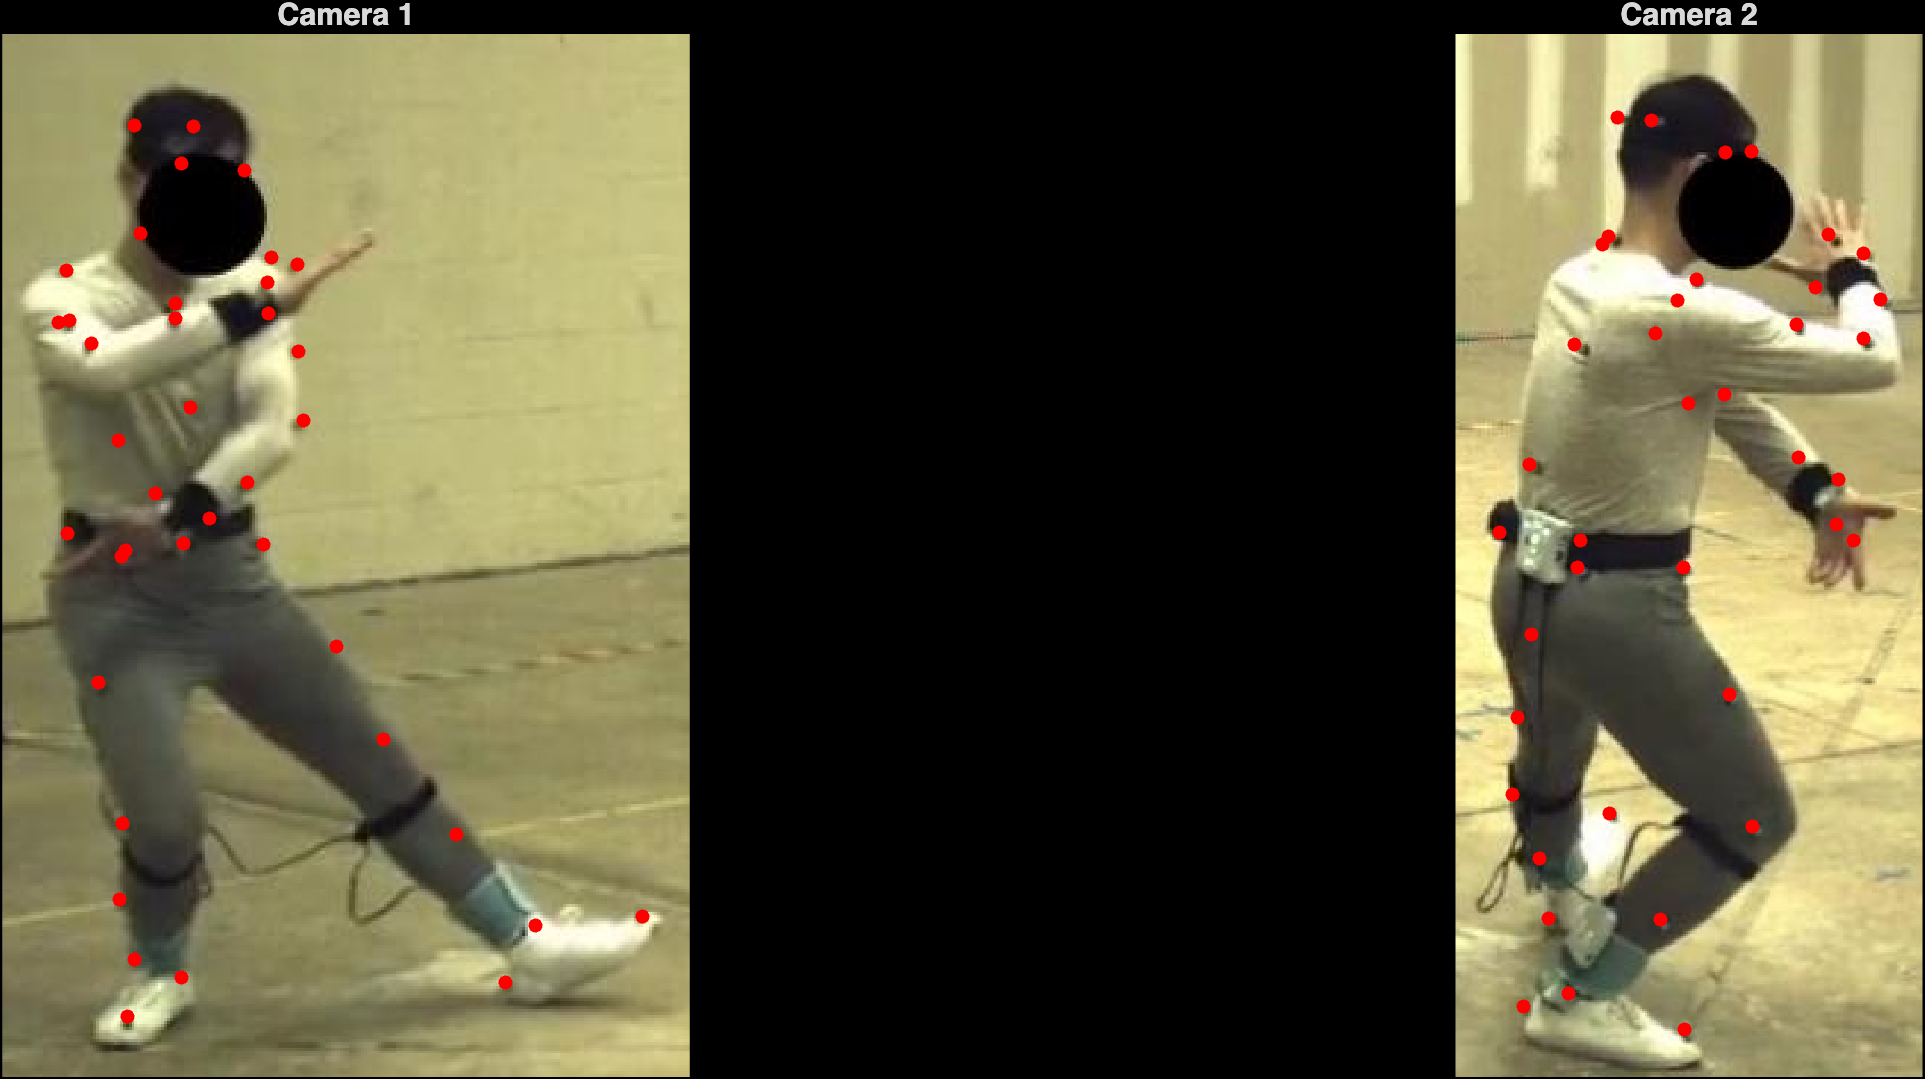
\includegraphics[width=0.8\linewidth]{extra1_projection.png}
    \caption{Projected mocap points on the cropped views of camera 1
    (left) and camera 2 (right), using the modified $K'$.}
    \label{fig:extra1-proj}
\end{figure}

\medskip

The points fall on the same body locations as in the full views, which
shows that the modified $K'$ matrices are correct.

\subsection*{Modified fundamental matrix}
We recompute the fundamental matrix with the function from Task 3.5, using the modified matrices $K_1'$ and $K_2'$:

\begin{center}
    $F' = K_2'^{-T}\,R\,S\,K_1'^{-1}$.
\end{center}

\medskip

The relative pose $R$ and $T$ do not
change, since cropping does not move the cameras. The result is:

\[
F' \approx
\begin{bmatrix}
-9.95\times10^{-6} & 2.02\times10^{-4} & 7.89\times10^{-3} \\
 2.39\times10^{-4} & 3.38\times10^{-5} & 0.344 \\
 0.0379 & -0.502 & -0.811
\end{bmatrix}.
\]

Figure~\ref{fig:extra1-epi} shows the epipolar lines for all 39 projected
points in both directions.

\begin{figure}[H]
    \centering
    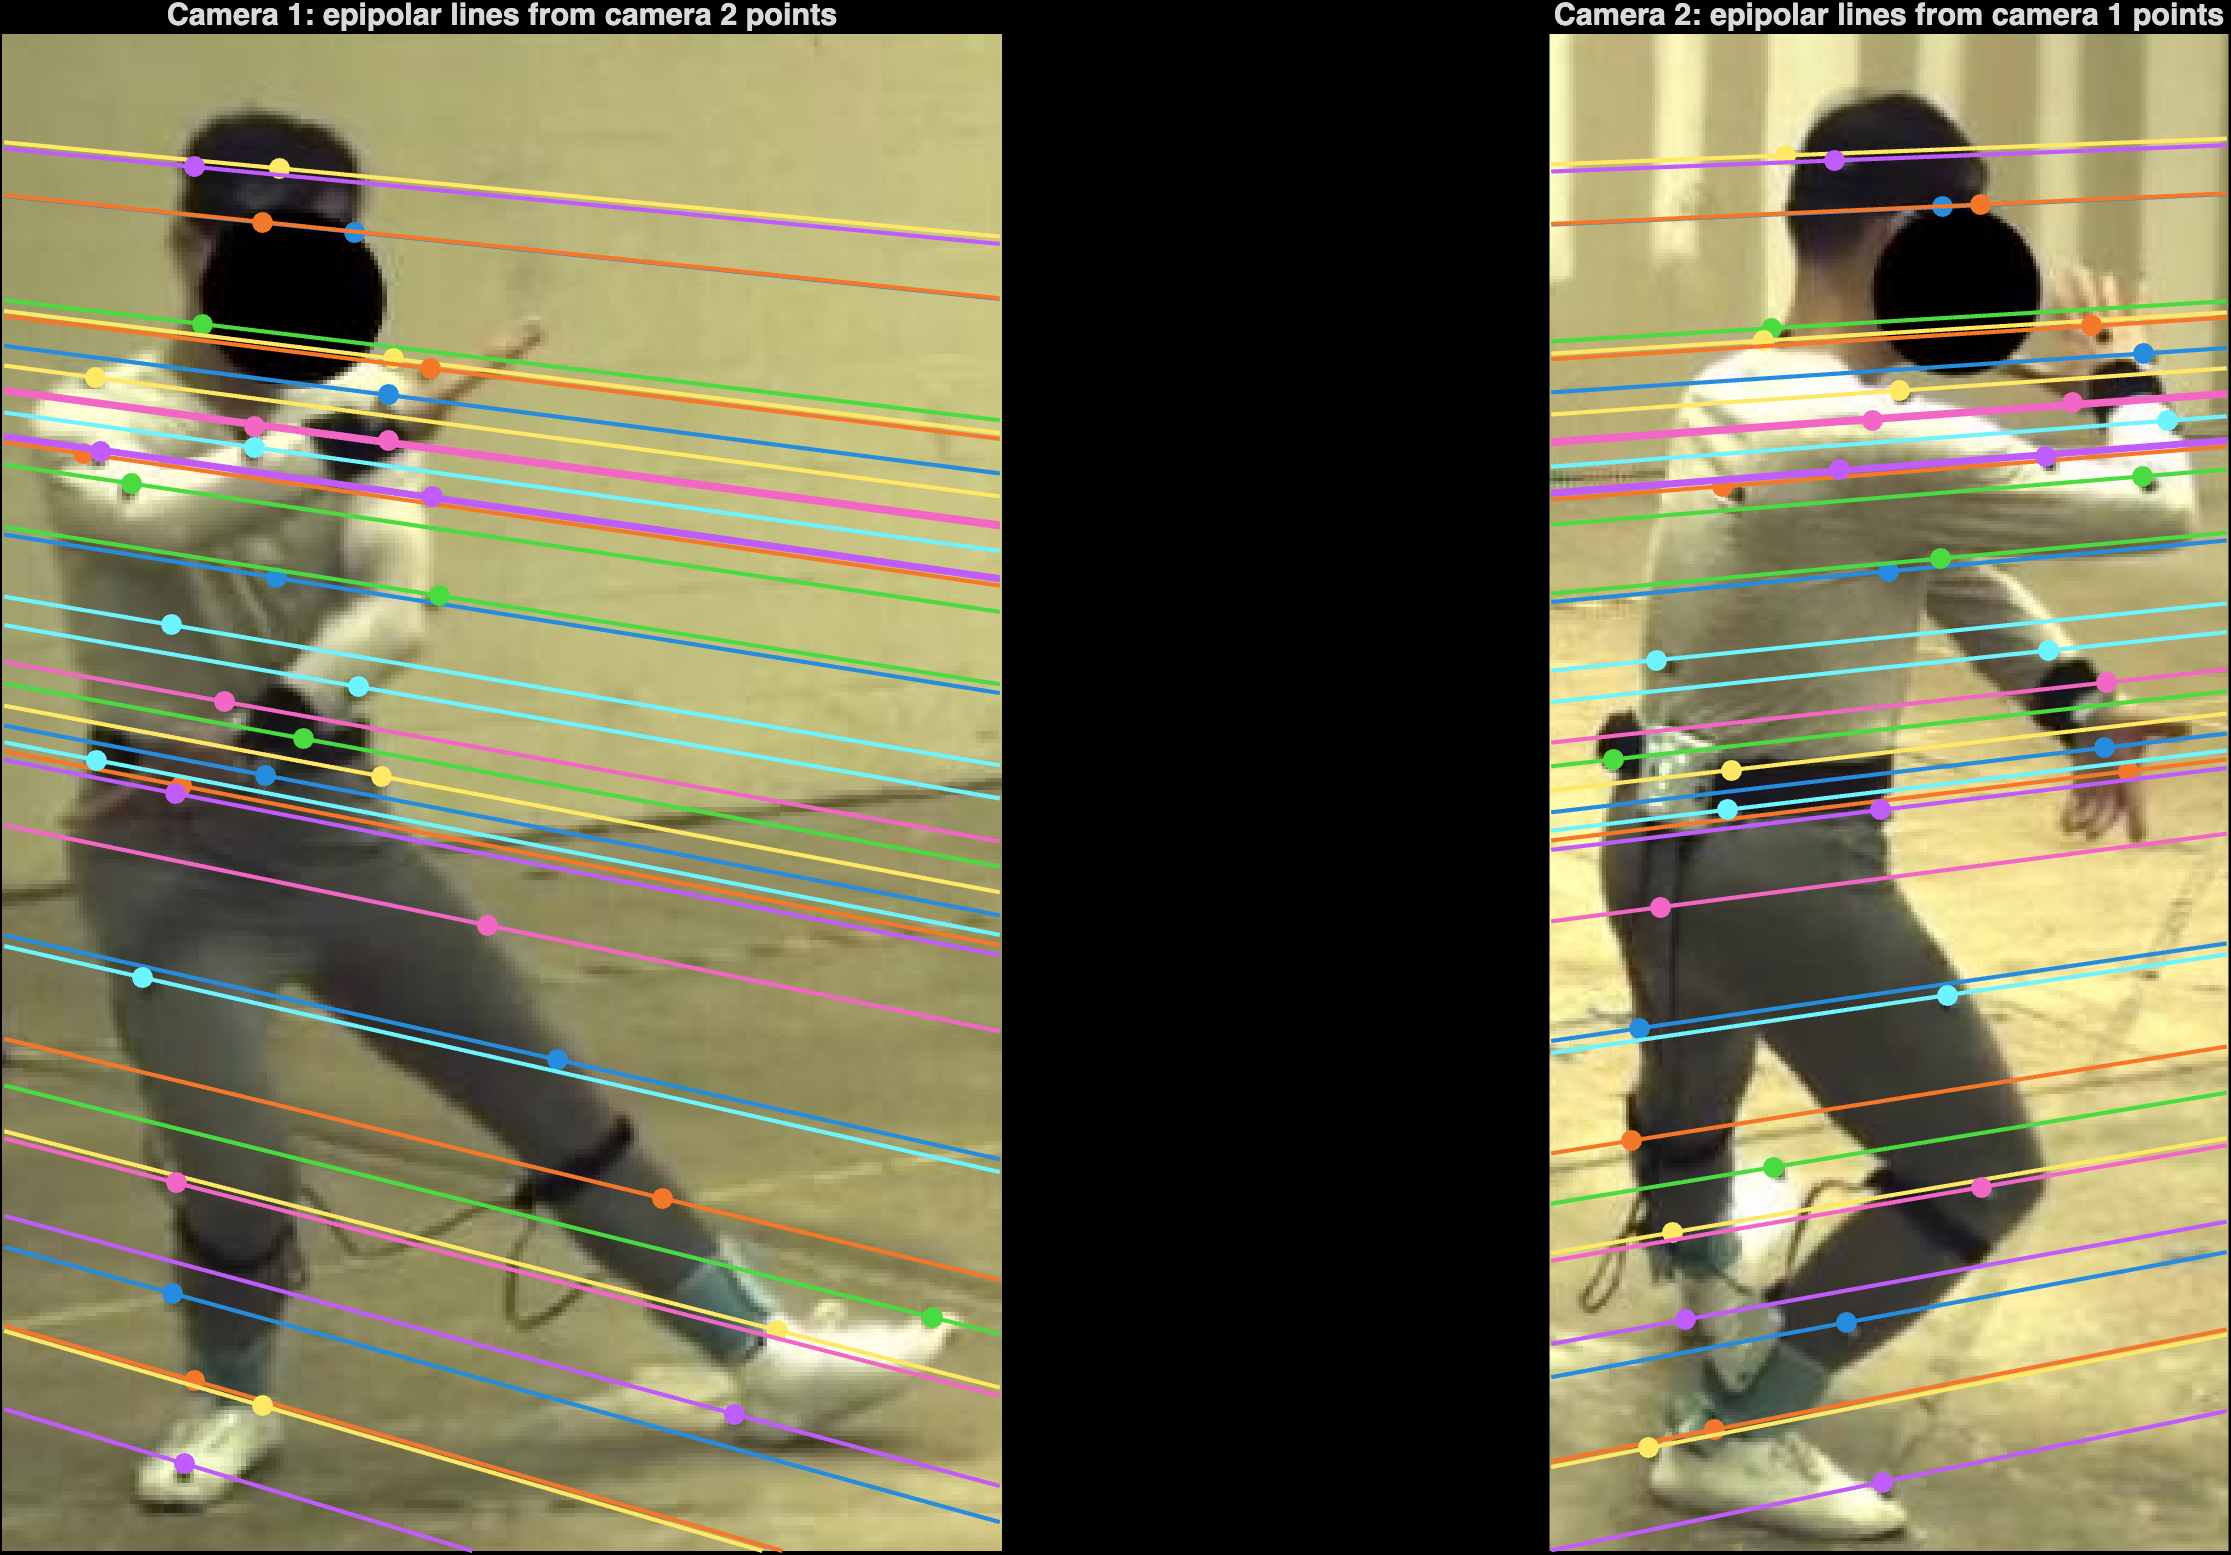
\includegraphics[width=0.8\linewidth]{extra1_epipolar.png}
    \caption{Epipolar lines from $F'$ on the cropped views. Each point
    lies on the line of the same color in the other image.}
    \label{fig:extra1-epi}
\end{figure}

Every point lies on its epipolar line in both views, so $F'$ correctly describes the epipolar geometry of the cropped images. 





\end{document}
